%%%%%%%%%%%%%%%%%%%%%%%%%%%%%%%%%%%%%%%%%
% Beamer Presentation
% LaTeX Template
% Version 2.0 (March 8, 2022)
%
% This template originates from:
% https://www.LaTeXTemplates.com
%
% Author:
% Vel (vel@latextemplates.com)
%
% License:
% CC BY-NC-SA 4.0 (https://creativecommons.org/licenses/by-nc-sa/4.0/)
%
%%%%%%%%%%%%%%%%%%%%%%%%%%%%%%%%%%%%%%%%%

%----------------------------------------------------------------------------------------
%	PACKAGES AND OTHER DOCUMENT CONFIGURATIONS
%----------------------------------------------------------------------------------------

\documentclass[
	10pt, % Set the default font size, options include: 8pt, 9pt, 10pt, 11pt, 12pt, 14pt, 17pt, 20pt
	%t, % Uncomment to vertically align all slide content to the top of the slide, rather than the default centered
	%aspectratio=169, % Uncomment to set the aspect ratio to a 16:9 ratio which matches the aspect ratio of 1080p and 4K screens and projectors
]{beamer}

\graphicspath{{figures/}{./}} % Specifies where to look for included images (trailing slash required)


\usepackage{booktabs} % Allows the use of \toprule, \midrule and \bottomrule for better rules in tables
\usepackage{multimedia}
\usepackage{hyperref}
%----------------------------------------------------------------------------------------
%	SELECT LAYOUT THEME
%----------------------------------------------------------------------------------------

% Beamer comes with a number of default layout themes which change the colors and layouts of slides. Below is a list of all themes available, uncomment each in turn to see what they look like.

%\usetheme{default}
%\usetheme{AnnArbor}
%\usetheme{Antibes}
%\usetheme{Bergen}
%\usetheme{Berkeley}
%\usetheme{Berlin}
%\usetheme{Boadilla}
%\usetheme{CambridgeUS}
%\usetheme{Copenhagen}
%\usetheme{Darmstadt}
%\usetheme{Dresden}
%\usetheme{Frankfurt}
%\usetheme{Goettingen}
%\usetheme{Hannover}
%\usetheme{Ilmenau}
%\usetheme{JuanLesPins}
%\usetheme{Luebeck}
\usetheme{Madrid}
%\usetheme{Malmoe}
%\usetheme{Marburg}
%\usetheme{Montpellier}
%\usetheme{PaloAlto}
%\usetheme{Pittsburgh}
%\usetheme{Rochester}
%\usetheme{Singapore}
%\usetheme{Szeged}
%\usetheme{Warsaw}

%----------------------------------------------------------------------------------------
%	SELECT COLOR THEME
%----------------------------------------------------------------------------------------

% Beamer comes with a number of color themes that can be applied to any layout theme to change its colors. Uncomment each of these in turn to see how they change the colors of your selected layout theme.

% \usecolortheme{albatross}
%\usecolortheme{beaver}
%\usecolortheme{beetle}
%\usecolortheme{crane}
%\usecolortheme{dolphin}
%\usecolortheme{dove}
%\usecolortheme{fly}
%\usecolortheme{lily}
%\usecolortheme{monarca}
%\usecolortheme{seagull}
%\usecolortheme{seahorse}
%\usecolortheme{spruce}
%\usecolortheme{whale}
% \usecolortheme{wolverine}

%----------------------------------------------------------------------------------------
%	SELECT FONT THEME & FONTS
%----------------------------------------------------------------------------------------

% Beamer comes with several font themes to easily change the fonts used in various parts of the presentation. Review the comments beside each one to decide if you would like to use it. Note that additional options can be specified for several of these font themes, consult the beamer documentation for more information.

\usefonttheme{default} % Typeset using the default sans serif font
%\usefonttheme{serif} % Typeset using the default serif font (make sure a sans font isn't being set as the default font if you use this option!)
%\usefonttheme{structurebold} % Typeset important structure text (titles, headlines, footlines, sidebar, etc) in bold
%\usefonttheme{structureitalicserif} % Typeset important structure text (titles, headlines, footlines, sidebar, etc) in italic serif
%\usefonttheme{structuresmallcapsserif} % Typeset important structure text (titles, headlines, footlines, sidebar, etc) in small caps serif

%------------------------------------------------

%\usepackage{mathptmx} % Use the Times font for serif text
\usepackage{palatino} % Use the Palatino font for serif text

%\usepackage{helvet} % Use the Helvetica font for sans serif text
\usepackage[default]{opensans} % Use the Open Sans font for sans serif text
%\usepackage[default]{FiraSans} % Use the Fira Sans font for sans serif text
%\usepackage[default]{lato} % Use the Lato font for sans serif text

%----------------------------------------------------------------------------------------
%	SELECT INNER THEME
%----------------------------------------------------------------------------------------

% Inner themes change the styling of internal slide elements, for example: bullet points, blocks, bibliography entries, title pages, theorems, etc. Uncomment each theme in turn to see what changes it makes to your presentation.

%\useinnertheme{default}
\useinnertheme{circles}
%\useinnertheme{rectangles}
%\useinnertheme{rounded}
%\useinnertheme{inmargin}

%----------------------------------------------------------------------------------------
%	SELECT OUTER THEME
%----------------------------------------------------------------------------------------

% Outer themes change the overall layout of slides, such as: header and footer lines, sidebars and slide titles. Uncomment each theme in turn to see what changes it makes to your presentation.

%\useoutertheme{default}
%\useoutertheme{infolines}
%\useoutertheme{miniframes}
%\useoutertheme{smoothbars}
%\useoutertheme{sidebar}
%\useoutertheme{split}
%\useoutertheme{shadow}
%\useoutertheme{tree}
%\useoutertheme{smoothtree}

%\setbeamertemplate{footline} % Uncomment this line to remove the footer line in all slides
%\setbeamertemplate{footline}[page number] % Uncomment this line to replace the footer line in all slides with a simple slide count

%\setbeamertemplate{navigation symbols}{} % Uncomment this line to remove the navigation symbols from the bottom of all slides

%----------------------------------------------------------------------------------------
%	PRESENTATION INFORMATION
%----------------------------------------------------------------------------------------

\title[Master's thesis midway presentation]{Tuning frictional properties of graphene sheets using kirigami inspired cuts and inverse design} % The short title in the optional parameter appears at the bottom of every slide, the full title in the main parameter is only on the title page

% \subtitle{Optional Subtitle} % Presentation subtitle, remove this command if a subtitle isn't required

\author[Mikkel Metzsch Jensen]{Mikkel Metzsch Jensen} % Presenter name(s), the optional parameter can contain a shortened version to appear on the bottom of every slide, while the main parameter will appear on the title slide

\institute[UiO]{Universitetet i Oslo} % Your institution, the optional parameter can be used for the institution shorthand and will appear on the bottom of every slide after author names, while the required parameter is used on the title slide and can include your email address or additional information on separate lines

\date[\today]{Master's thesis midway presentation \\ November 29, 2022} % Presentation date or conference/meeting name, the optional parameter can contain a shortened version to appear on the bottom of every slide, while the required parameter value is output to the title slide

%----------------------------------------------------------------------------------------

\begin{document}

%----------------------------------------------------------------------------------------
%	TITLE SLIDE
%----------------------------------------------------------------------------------------

\begin{frame}
	\titlepage % Output the title slide, automatically created using the text entered in the PRESENTATION INFORMATION block above
\end{frame}

%----------------------------------------------------------------------------------------
%	TABLE OF CONTENTS SLIDE
%----------------------------------------------------------------------------------------

% The table of contents outputs the sections and subsections that appear in your presentation, specified with the standard \section and \subsection commands. You may either display all sections and subsections on one slide with \tableofcontents, or display each section at a time on subsequent slides with \tableofcontents[pausesections]. The latter is useful if you want to step through each section and mention what you will discuss.

% \begin{frame}
% 	\frametitle{Presentation Overview} % Slide title, remove this command for no title
	
% 	\tableofcontents % Output the table of contents (all sections on one slide)
% 	%\tableofcontents[pausesections] % Output the table of contents (break sections up across separate slides)
% \end{frame}

%----------------------------------------------------------------------------------------
%	PRESENTATION BODY SLIDES
%----------------------------------------------------------------------------------------


\section{Introduction}

\begin{frame}
	\frametitle{Project description}
	\framesubtitle{3 stages}


	\begin{enumerate}
		\setlength\itemsep{2em}
		\item \underline{Sheet kirigami}: Alter graphene sheet using atomic scale cuts. % Buckling in the 3rd dimension
		\item \underline{Forward simulation}: Calculate frictional properties of the sheet using MD simulations.
		\item \underline{Inverse design}: Predict cut patterns based on frictional properties and optimize for desired properties using machine learning.
		\begin{itemize}
			\item Low / high friction coefficient.
			\item Coupling between stretch and friction.
		\end{itemize} 
	

	\end{enumerate}

	
\end{frame}

\begin{frame}
	\frametitle{Motivation}
	\framesubtitle{Kirigami inspired cuts}

	Kirigami: Variation of origami with cuts permitted.

	\begin{figure}
		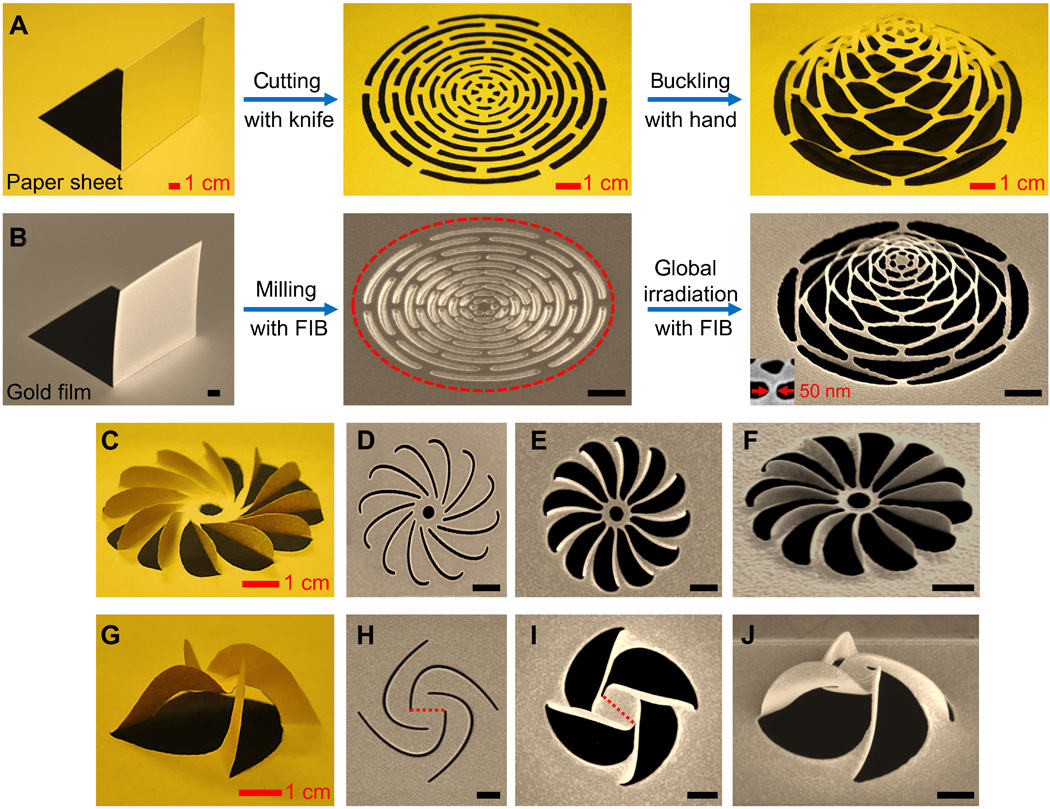
\includegraphics[width=0.6\linewidth]{figures/kirigami_example.jpeg}
		\caption{Example of transistion from macro- to nano-kirigami using a focused ion-beam (FIB) (Nano-kirigami with giant optical chirality, ZHIGUANG LIU, 2018).}
	\end{figure}	

\end{frame}

\begin{frame}
	\frametitle{Motivation}
	\framesubtitle{Kirigami inspired cuts}

	


	\begin{columns}[t] % The "c" option specifies centered vertical alignment while the "t" option is used for top vertical alignment
		\begin{column}{0.35\textwidth} % Left column width
			\newline
			\newline
			\textit{Accelerated Search and Design of Stretchable Graphene Kirigami Using Machine Learning, Paul Z. Hanakata, 2018.} \\
			% \hrulefill \\
			\begin{itemize}
				\item Kirigami inspired cuts is used to tune \textbf{yield stress} and \textbf{yield strain} as a function of cutting pattern.
				\item A side effect is buckling into the third dimension.
			\end{itemize}
		\end{column}
		\begin{column}{0.65\textwidth} % Right column width
			\vspace*{-0.7cm}
			\begin{figure}
				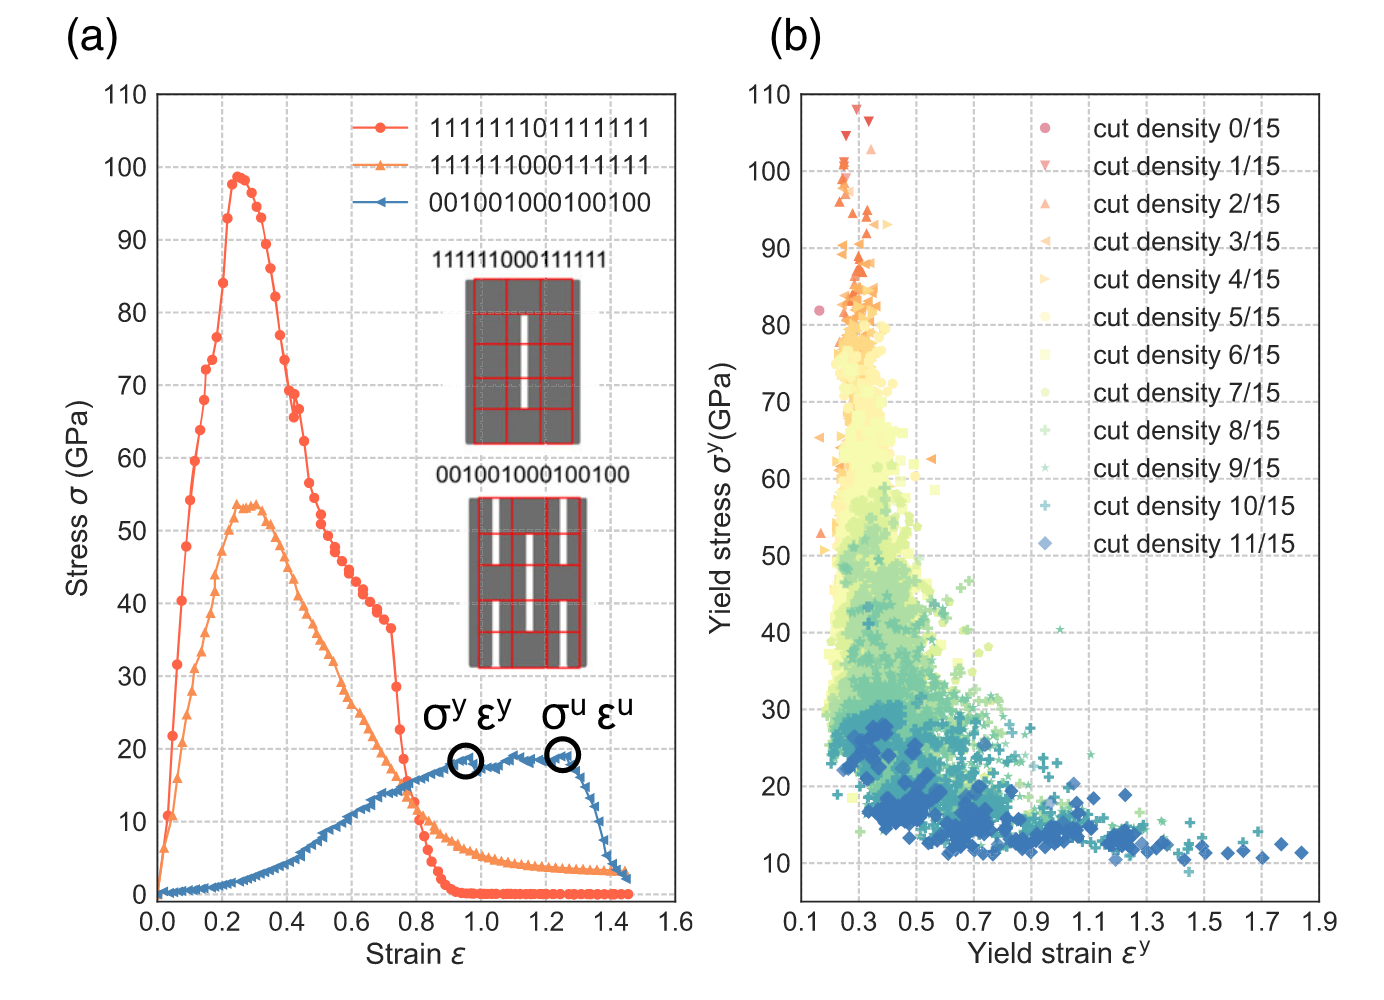
\includegraphics[width=\linewidth]{Hanakata2.png}
				\caption{(a) Stress-strain plot of three representative kirigamis. Inset shows the “typical” kirigami cuts. (b) Yield stress as a function of yield strain for different configurations.}
			\end{figure}
		\end{column}
	\end{columns}

	% \begin{columns}[c] % The "c" option specifies centered vertical alignment while the "t" option is used for top vertical alignment
	% 	\begin{column}{0.4\textwidth} % Left column width
	% 		\begin{figure}
	% 			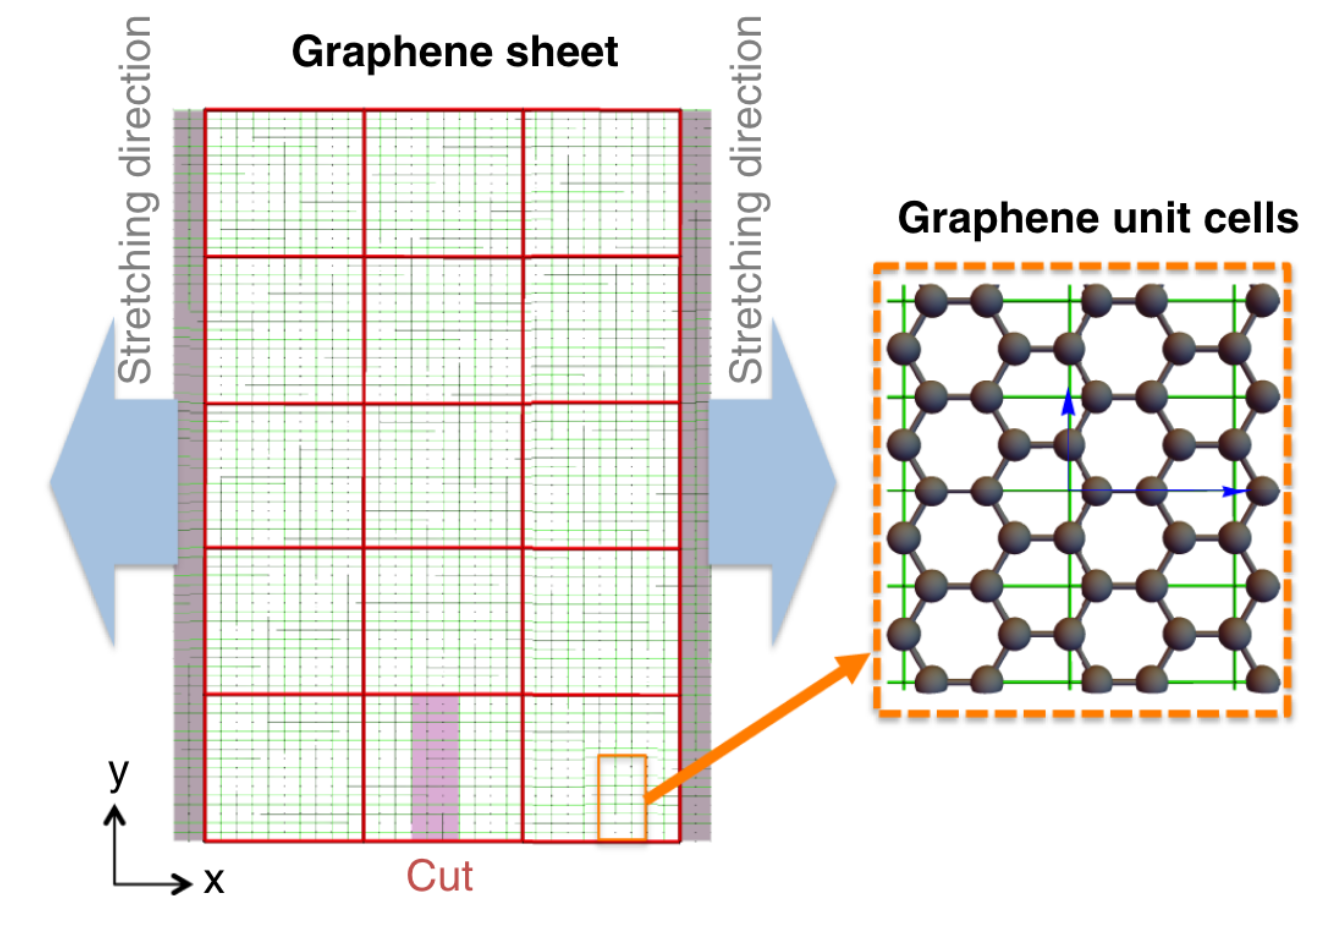
\includegraphics[width=\linewidth]{Hanakata1.png}
	% 			\caption{Schematic diagrams of a graphene sheet and rectangular graphene unit cells.}
	% 		\end{figure}
	% 	\end{column}
	% 	\begin{column}{0.6\textwidth} % Right column width
	% 		\begin{figure}
	% 			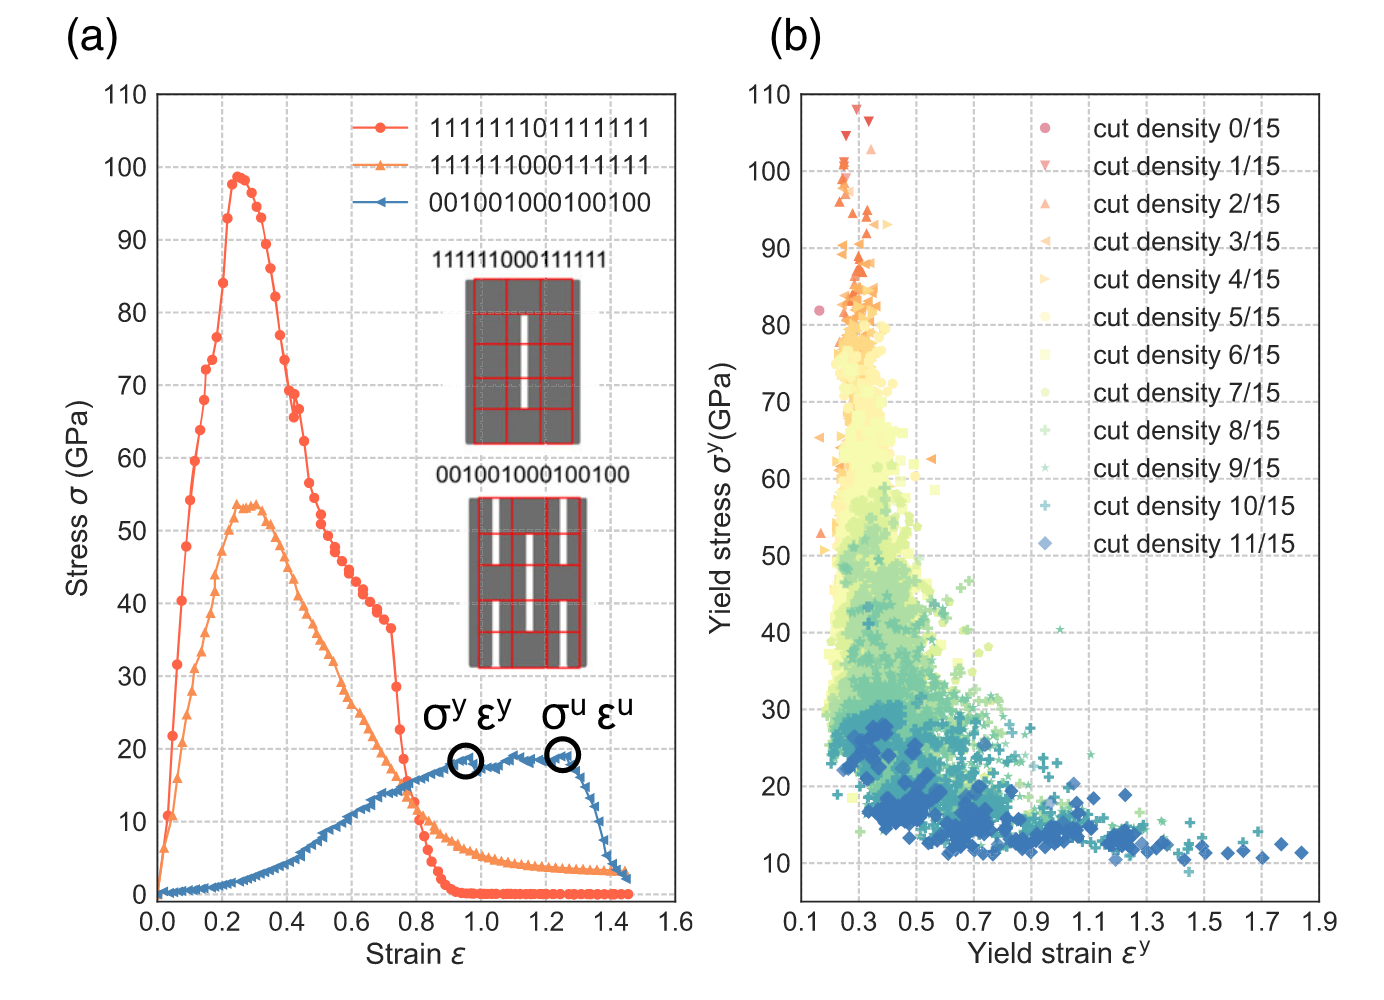
\includegraphics[width=\linewidth]{Hanakata2.png}
	% 			\caption{(a) Stress-strain plot of three representative kirigamis. Inset shows the “typical” kirigami cuts. (b) Yield stress as a function of yield strain for different configurations.}
	% 		\end{figure}
	% 	\end{column}
	% \end{columns}

\end{frame}


\begin{frame}
	\frametitle{Motivation}
	\framesubtitle{Friction laws}

	\begin{itemize}
		\item Friction laws at different scales:
		\begin{align*}
			\text{Microscopic: } &F_f = \mu \cdot F_N \quad (\text{ independent of } A), \\
			\text{Nanoscale: } &F_f \propto A = N_c \cdot A_c,  
		\end{align*}
		where $F_f$ is friction force, $\mu$ is the friction coefficient, $F_N$ is the normal force, $A$ is the contact area and $N_c$ is the average number of atoms in contact with an average contact area $A_c$.
		
		
	\end{itemize}
	
\end{frame}


\begin{frame}
	\frametitle{Motivation}
	\framesubtitle{Nanomachine for negative friction coefficient}

	\begin{align*}
		\left.\begin{aligned}
			\text{Contact area} &: A_0 = k \cdot F_N \\
			\text{Kirigami} &: A = A_0 - s_1 \cdot \text{stretch} \\
			\text{Nanomachine}&: \text{stretch} = s_2 \cdot F_n
		  \end{aligned}\right\} \Longrightarrow F_f \propto A = \underbrace{(k - s_1 \cdot s_2)}_{\mu} \cdot F_N
	\end{align*}
	
	\begin{figure}
		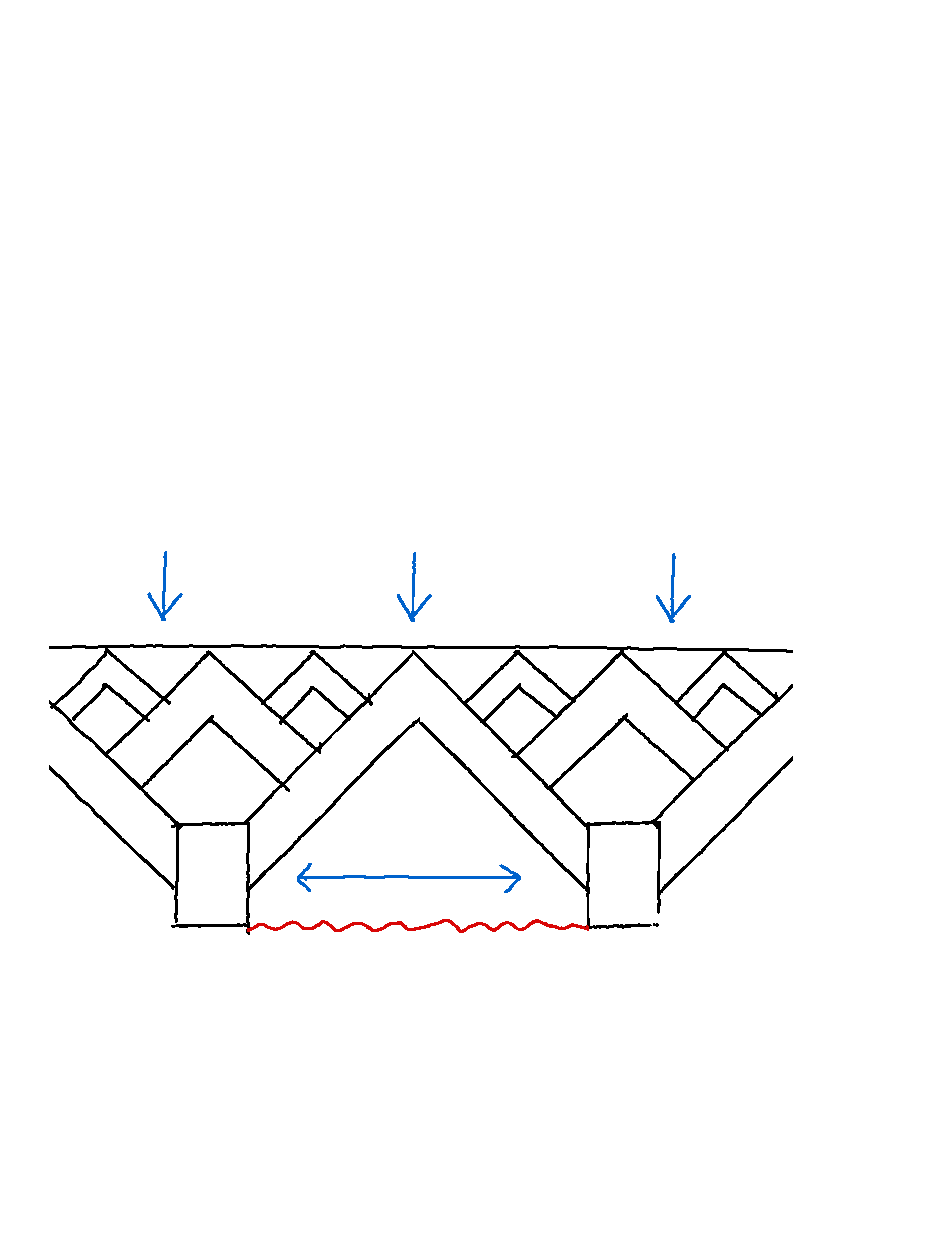
\includegraphics[width=0.6\linewidth]{figures/nanomachine.pdf}
		\caption{Sketch for nanomachine coupling normal force and stretch.}
	\end{figure}	

	
\end{frame}





\begin{frame}
	\frametitle{Motivation}
	\framesubtitle{Inverse design}
	\textit{Designing complex architectured materials with generative adversarial networks, YUNWEI MAO, 2020.}
	\begin{figure}
		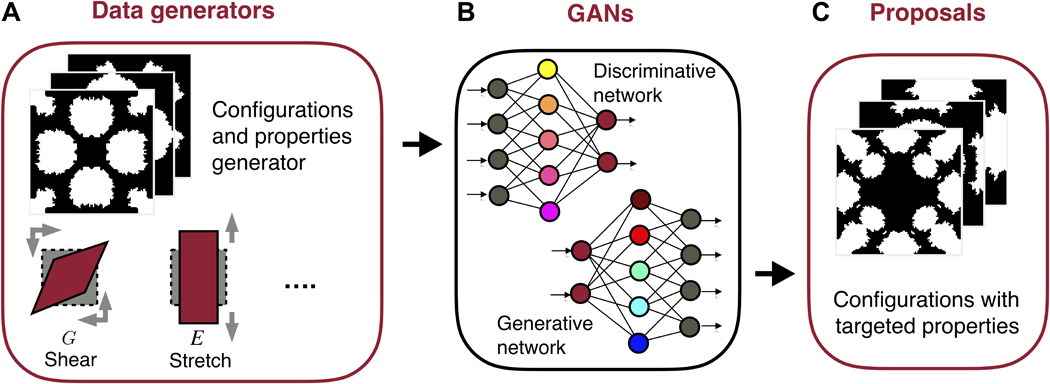
\includegraphics[width=0.8\linewidth]{figures/ML_procedure.jpeg}
		\caption{(A) Data generators to generate datasets of configurations and properties of architectured materials. (B) GANs trained by the datasets. (C) New designs of architectured materials with the targeted properties proposed by the GANs.}
	\end{figure}	

\end{frame}


% \begin{frame}
% 	\frametitle{Motivation}
% 	\framesubtitle{Inverse design}
% 	\begin{itemize}
% 		\item Inverse Design of Inflatable Soft Membranes Through Machine Learning
% 		\item Accelerated Search and Design of Stretchable Graphene Kirigami Using Machine Learning
% 		\item Designing complex architectured materials with generative adversarial networks
% 	\end{itemize}
% \end{frame}




%----------------------------------------------------------------------------------------
%	Further explanation / Development so far
%----------------------------------------------------------------------------------------



\begin{frame}
	\frametitle{Stage 1 - Kirigami cuts}
	\framesubtitle{Choosing a cut pattern}

	\begin{itemize}
		\item Kirigami design on macroscale.
	\end{itemize}
	\begin{figure}
		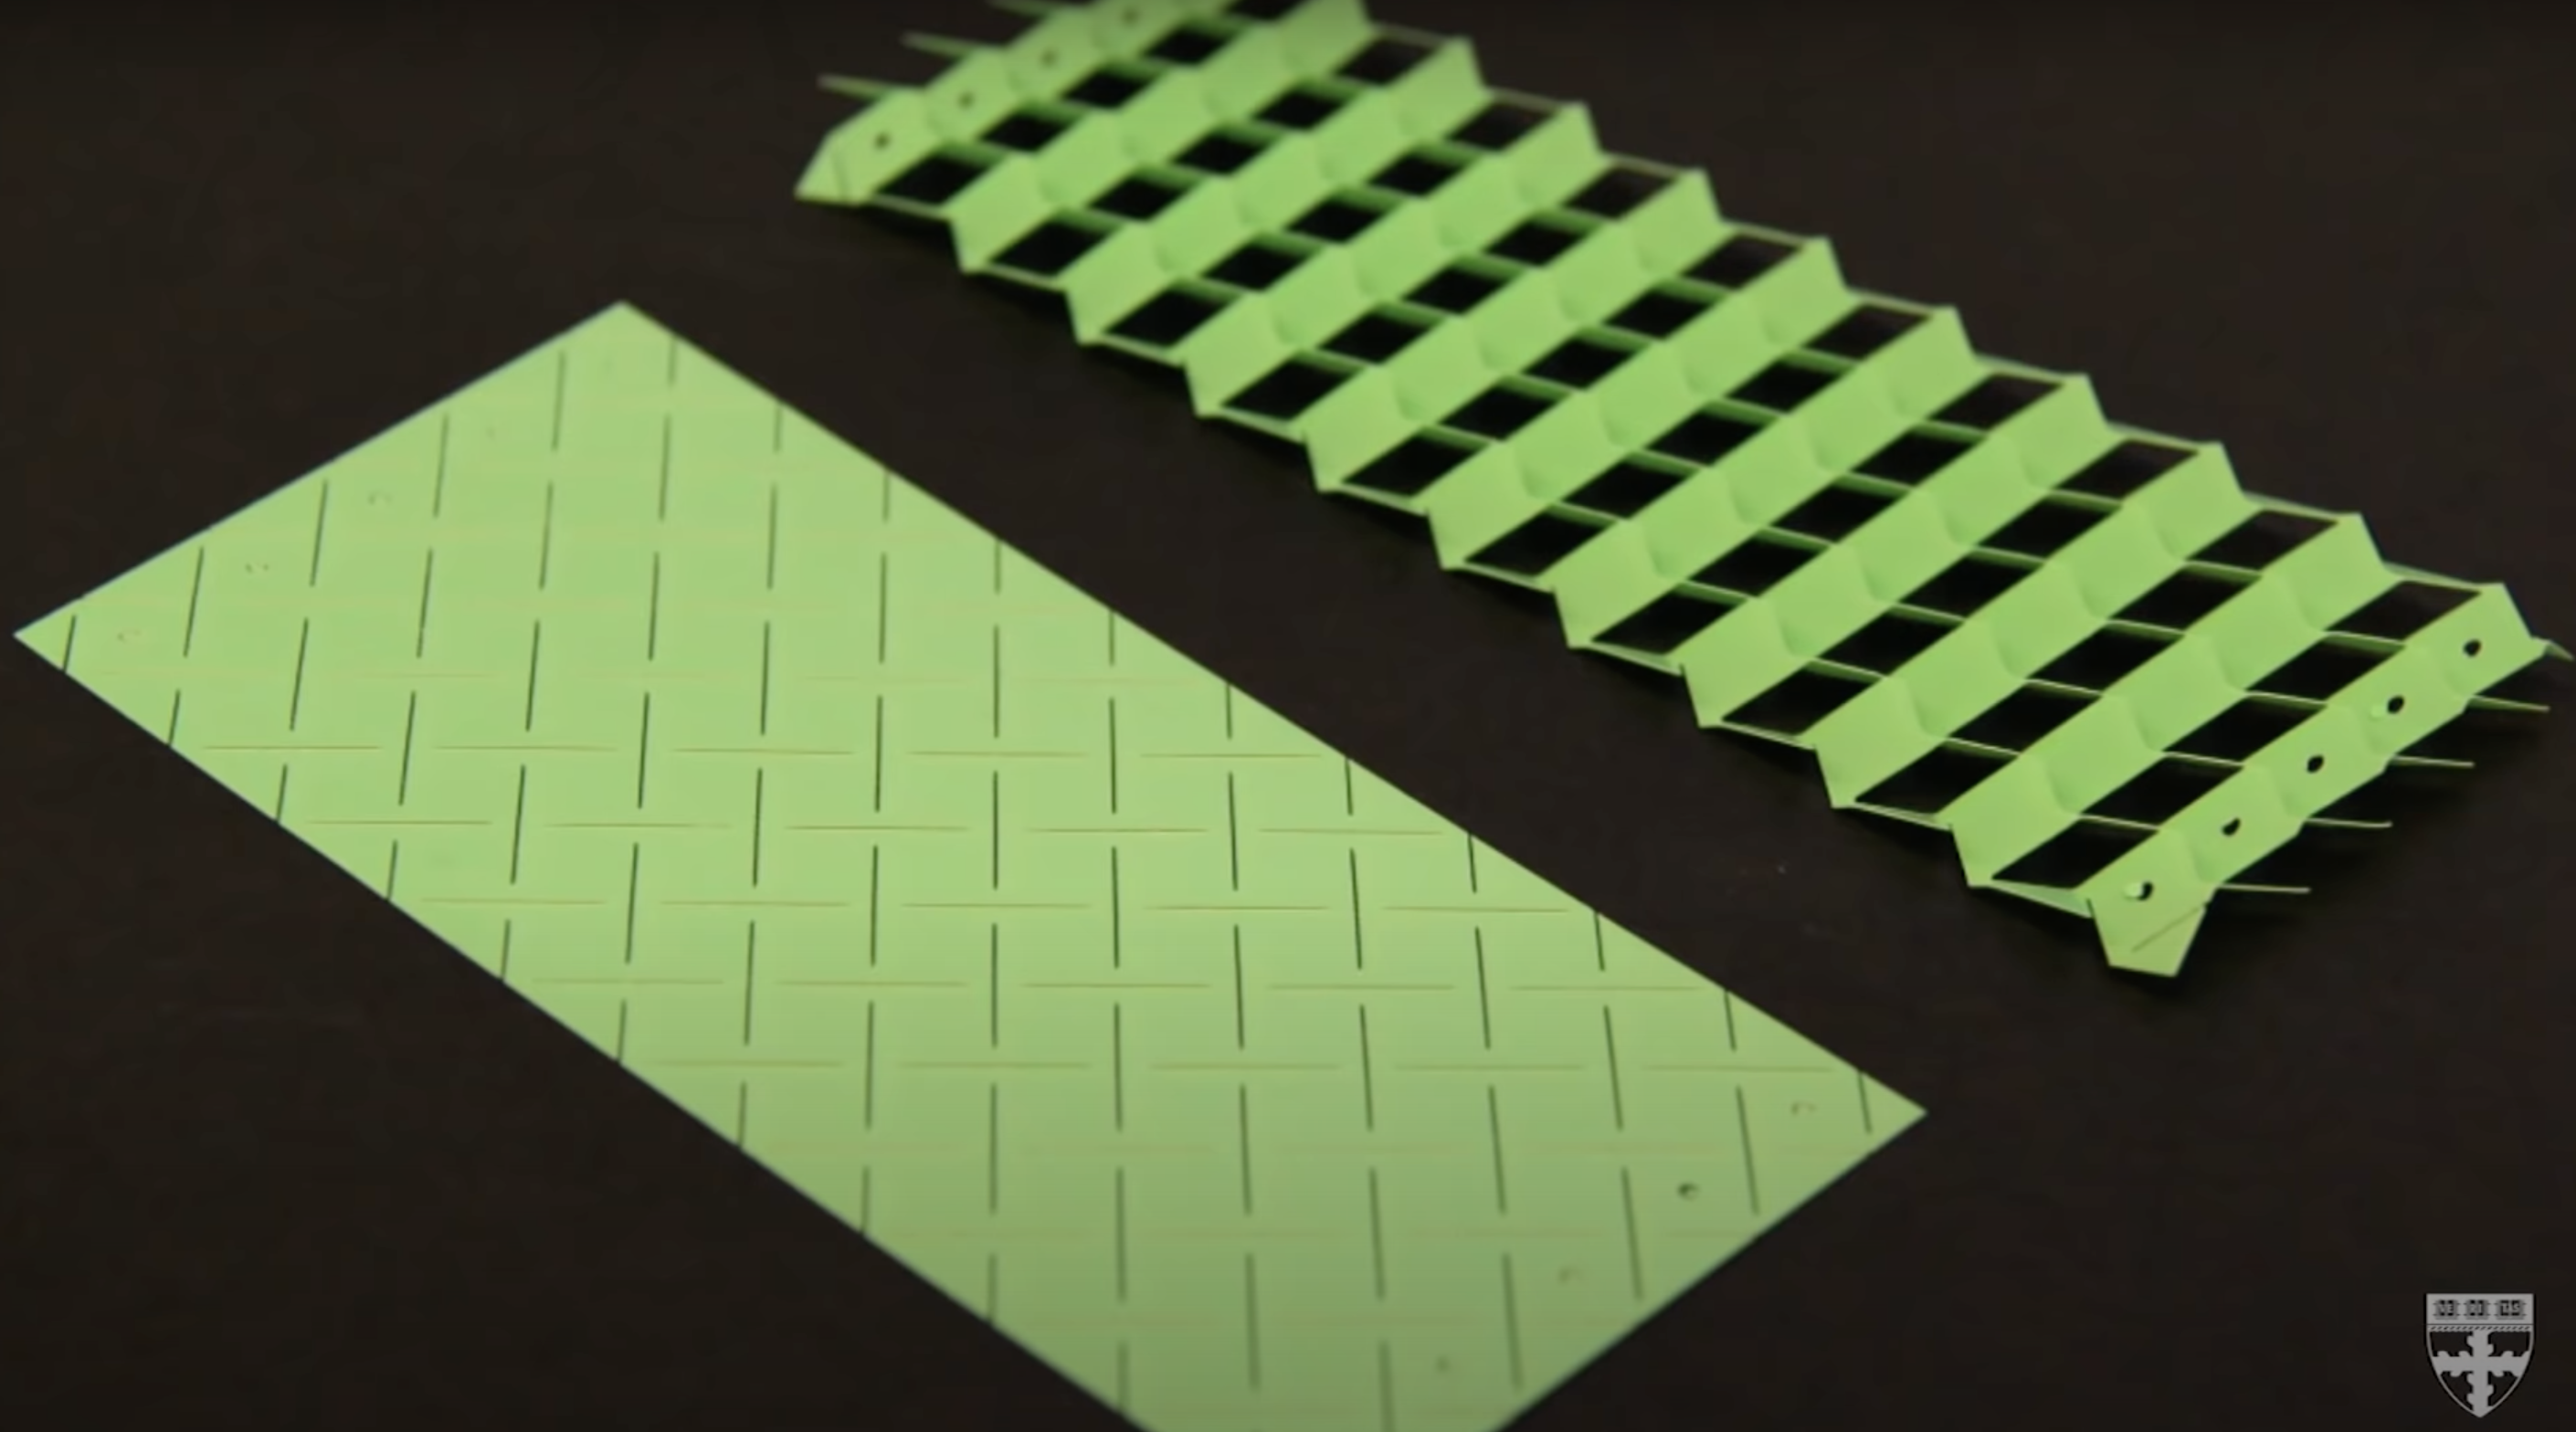
\includegraphics[width=0.6\linewidth]{figures/kirigami_pattern_inspiration.png}
		\caption{New pop-up strategy inspired by cuts, not folds - Leah Burrows, Harvard John A. Paulson School of Engineering and Applied Sciences.}
	\end{figure}	

	
\end{frame}



\begin{frame}
	\frametitle{Stage 1 - Kirigami cuts}
	\framesubtitle{Choosing a cut pattern}

	\begin{figure}
		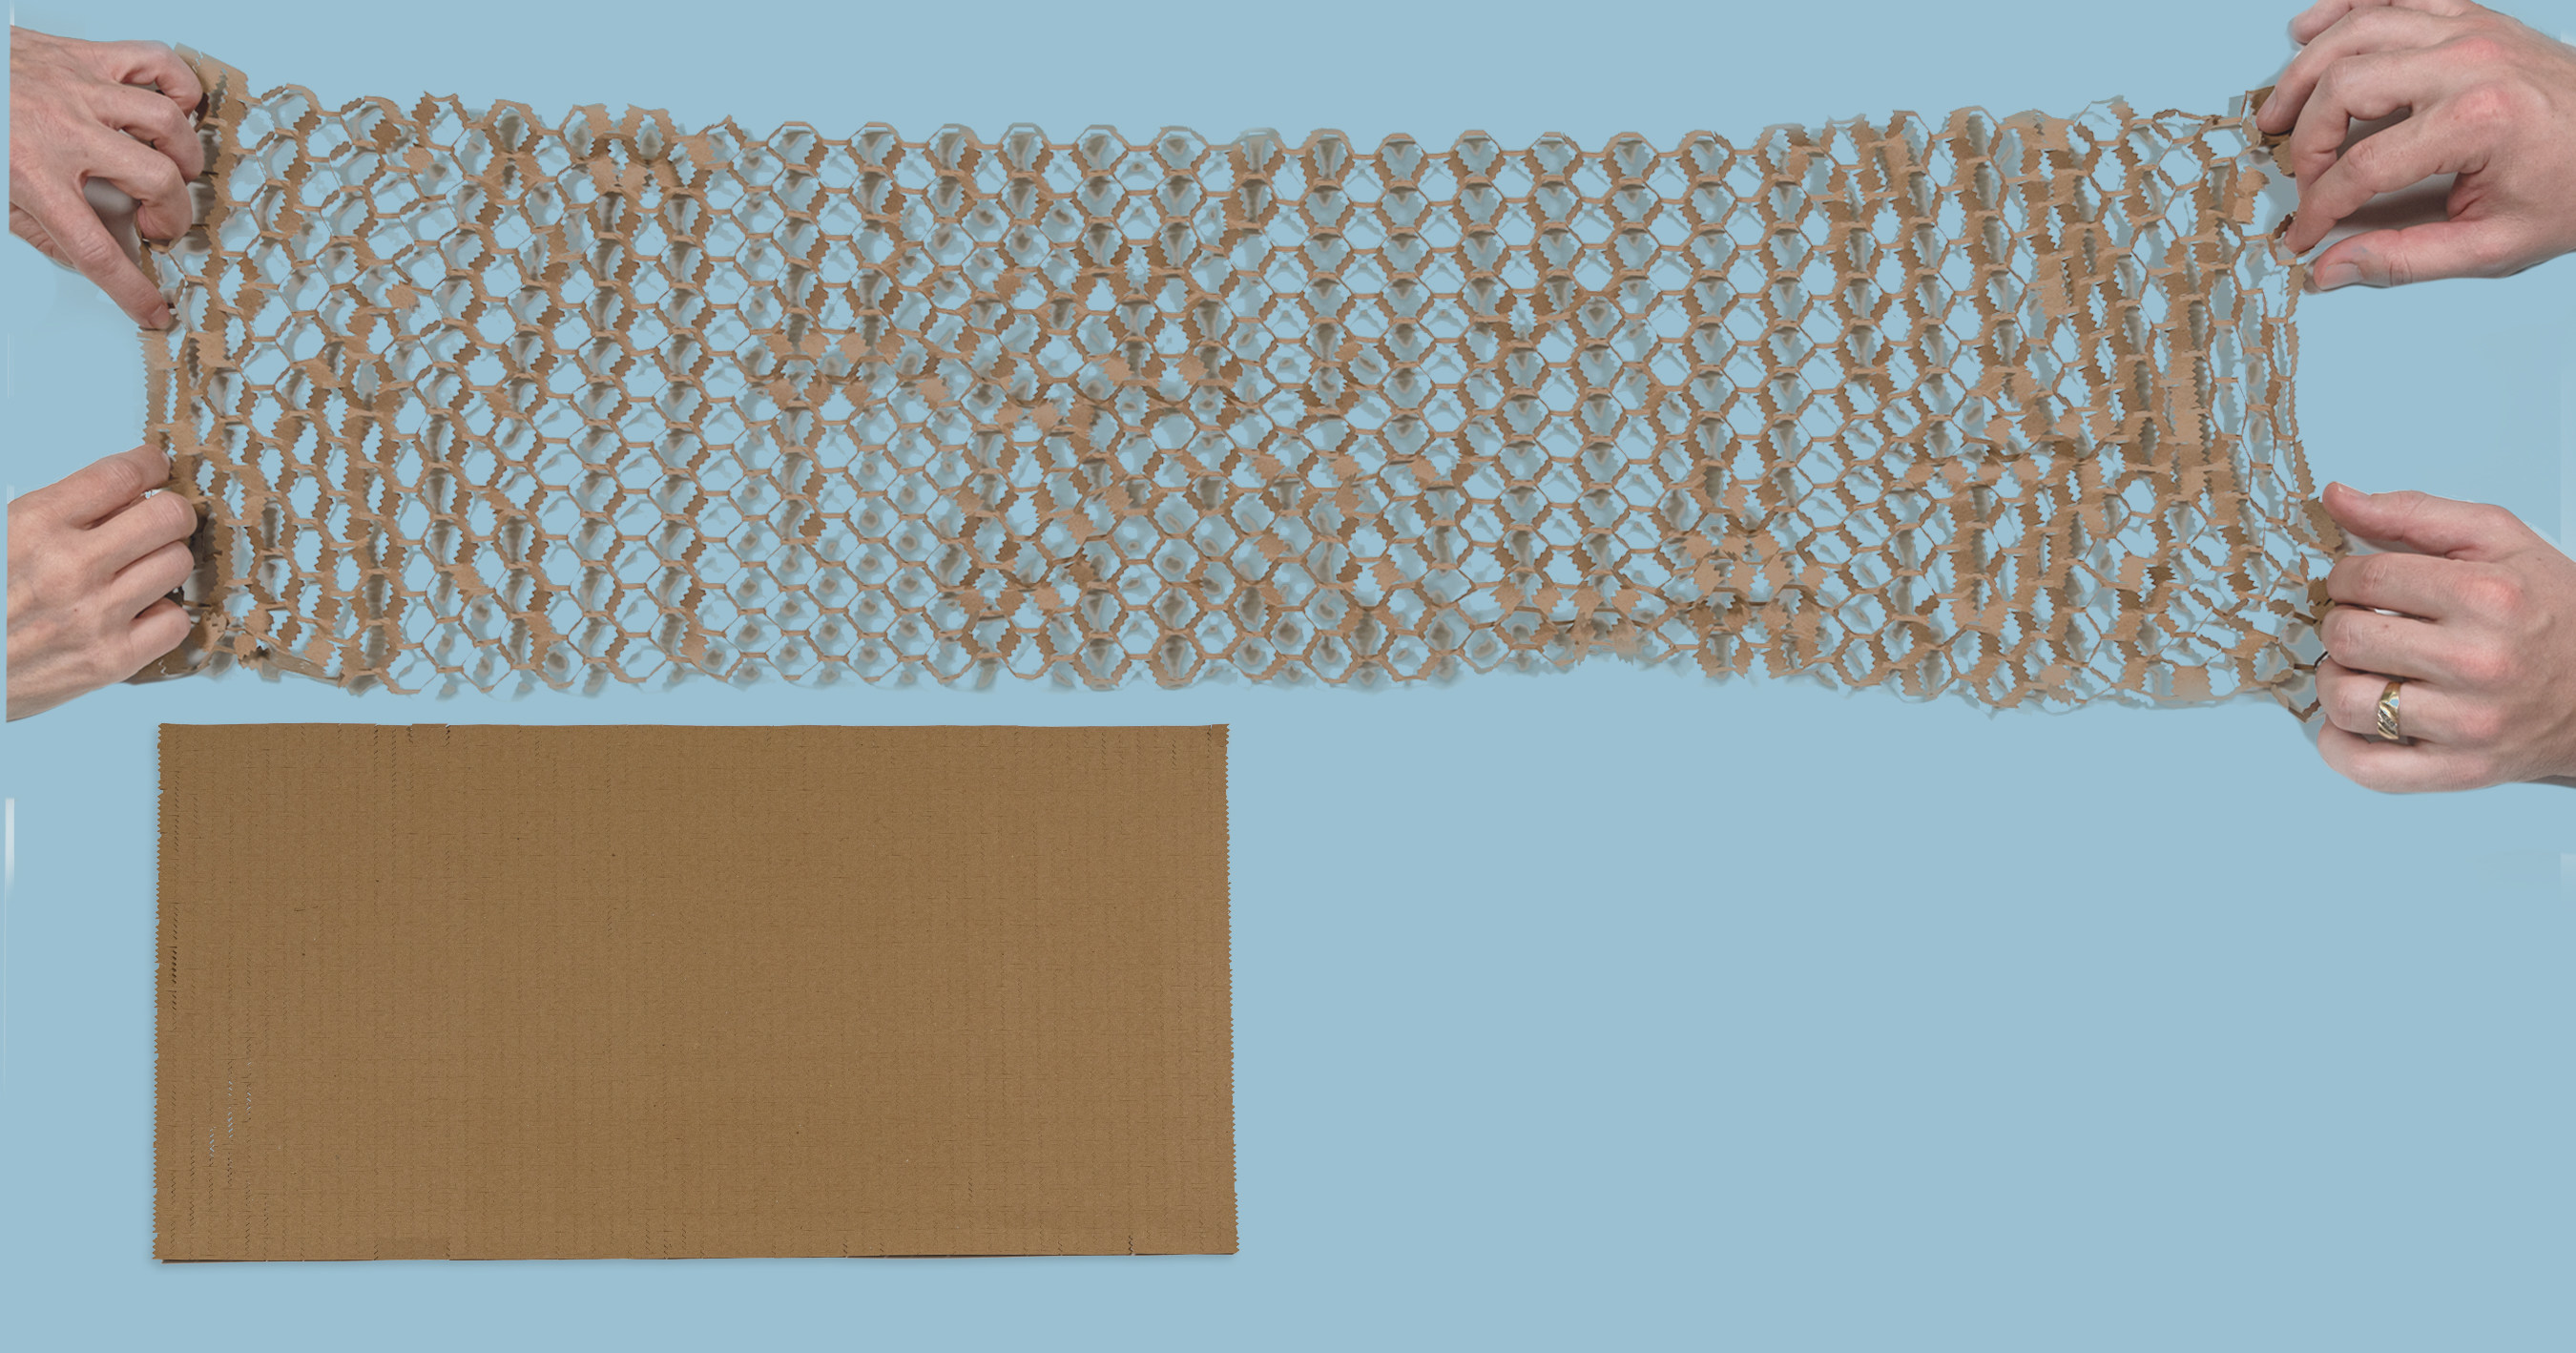
\includegraphics[width=0.8\linewidth]{figures/cushion_lock.jpg}
		\caption{Scotch Cushion Lock Protective Wrap.}
	\end{figure}	
	
\end{frame}



\begin{frame}
	\frametitle{Stage 1 - Kirigami cuts}
	\framesubtitle{Choosing a cut pattern}


	\begin{figure}
		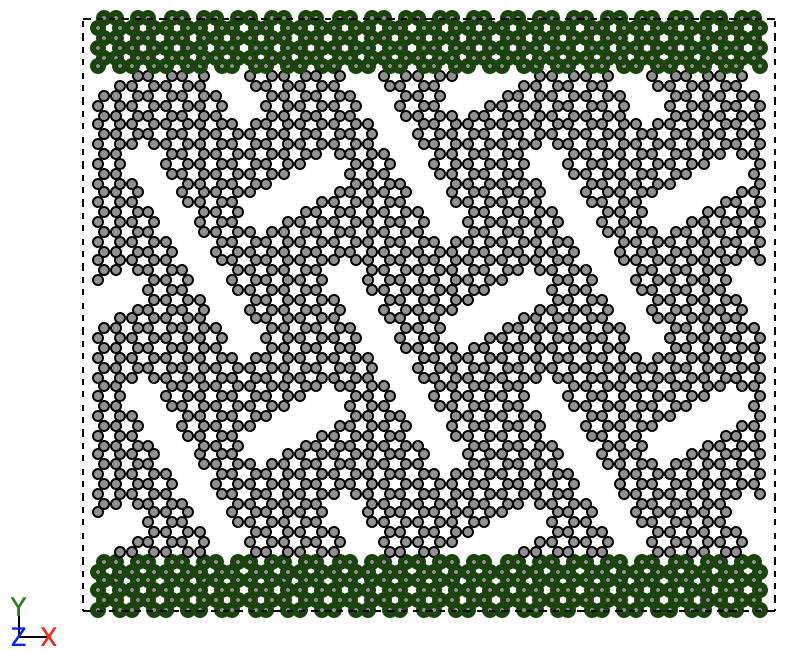
\includegraphics[width=0.6\linewidth]{figures/cutpattern.png}
		\caption{Example of cut pattern. The grey color marks the cutable sheet while green marks added blocks for stetching and dragging the sheet.}
	\end{figure}	

\end{frame}




\begin{frame}
	\frametitle{Stage 1 - Kirigami cuts}


	\begin{figure}
		\centering    
		\movie[open]{
\includegraphics[width=\textheight, keepaspectratio]{figures/vacuum_stretch.png}}{figures/vacuum_stretch.mov}
		\caption{Kirigami sheet stretch in vaccuum.}
   \end{figure} 

\end{frame}


\begin{frame}
	\frametitle{Stage 1 - Kirigami cuts}
	\framesubtitle{Investigating 3D buckling}
	
	\begin{figure}
		\centering    
		\movie[open]{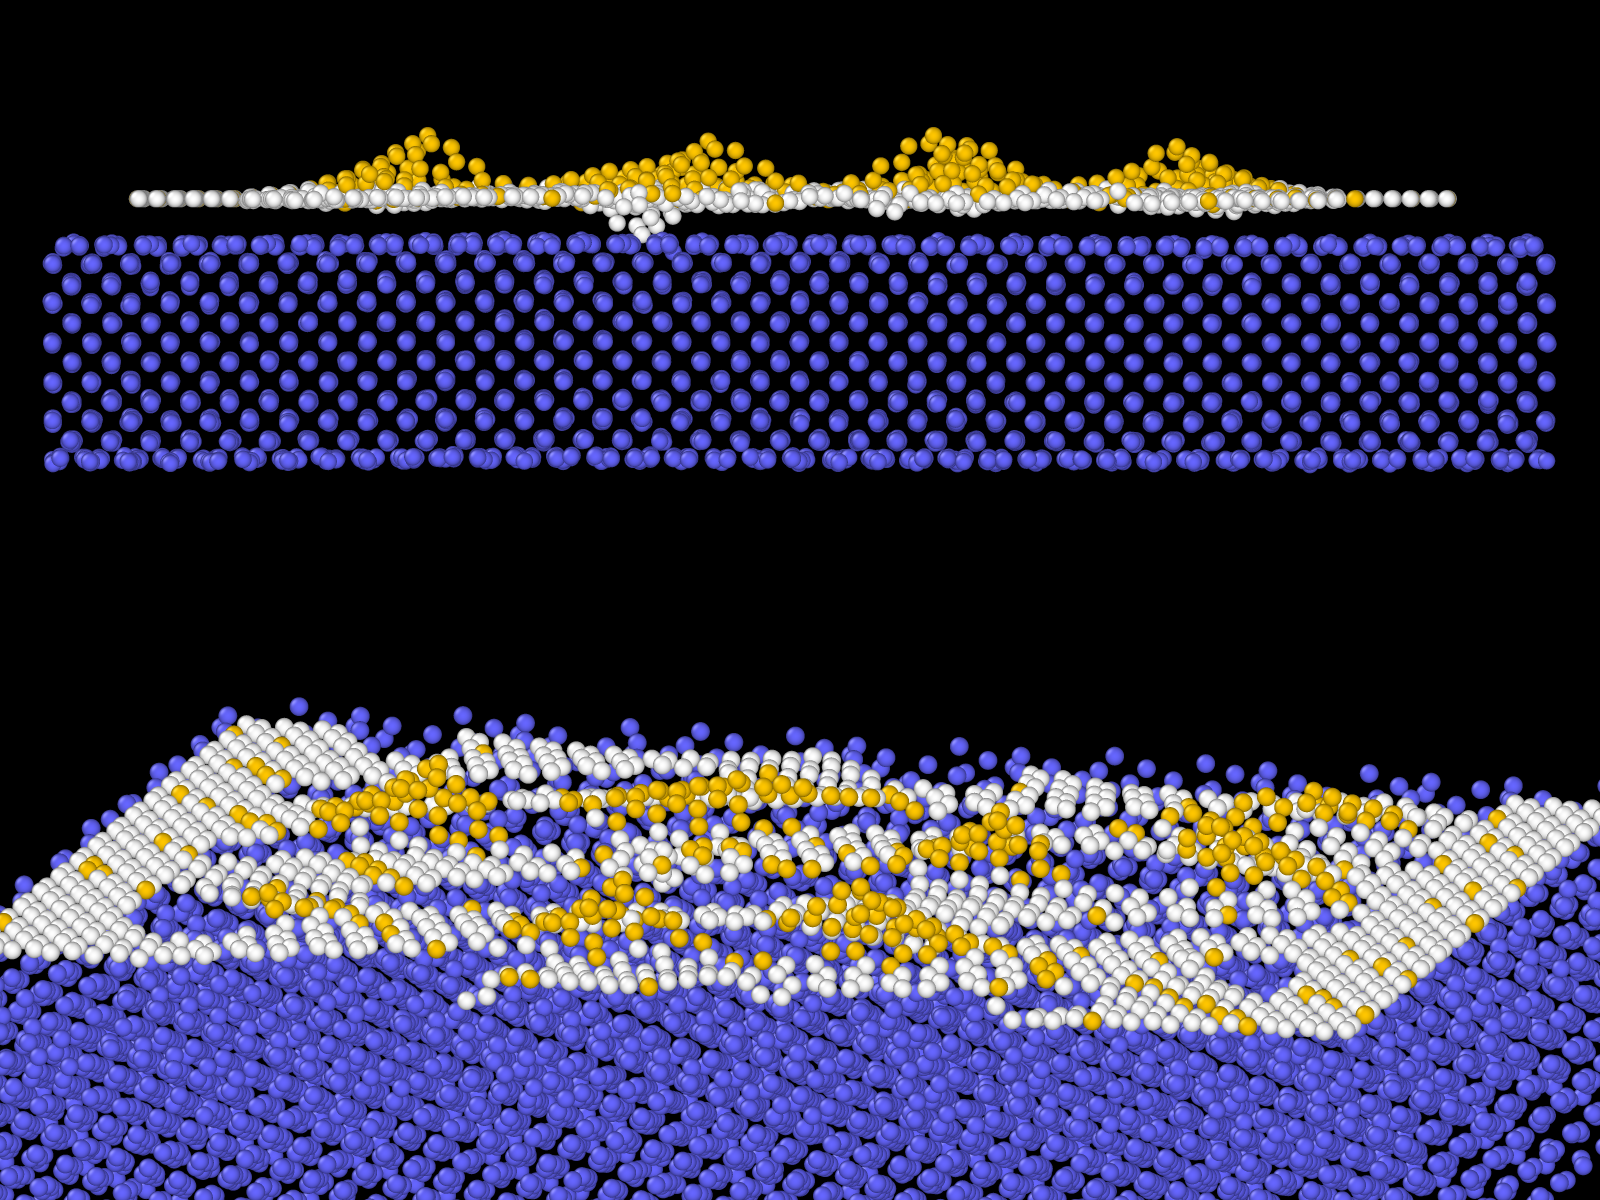
\includegraphics[width=0.95\textheight, keepaspectratio]{figures/contact_stretch.png}}{figures/contact_stretch.mov}
		\caption{Kirigami stretch in contact with Si-substrate.}
	\end{figure} 
	
	
	
\end{frame}


\begin{frame}
	\frametitle{Stage 1 - Kirigami cuts}
	\framesubtitle{Investigating 3D buckling}


	\begin{figure}
		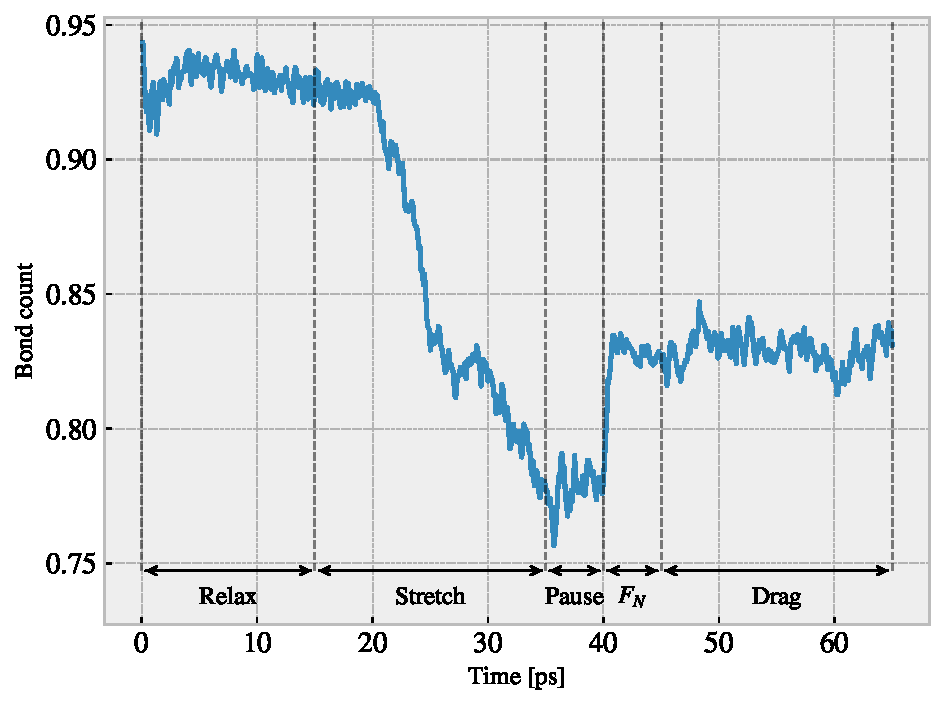
\includegraphics[width=0.7\linewidth]{figures/contact_pct.pdf}
		\caption{Contact area: number of C-Si bonds within a threshold distance of 110\% the equlibrium distance in LJ the potential.}
	\end{figure}	

	
\end{frame}


%------------------------------------------------

\begin{frame}
	\frametitle{Stage 2 - MD measurements}
	\framesubtitle{Friction force}

	
	\begin{figure}
		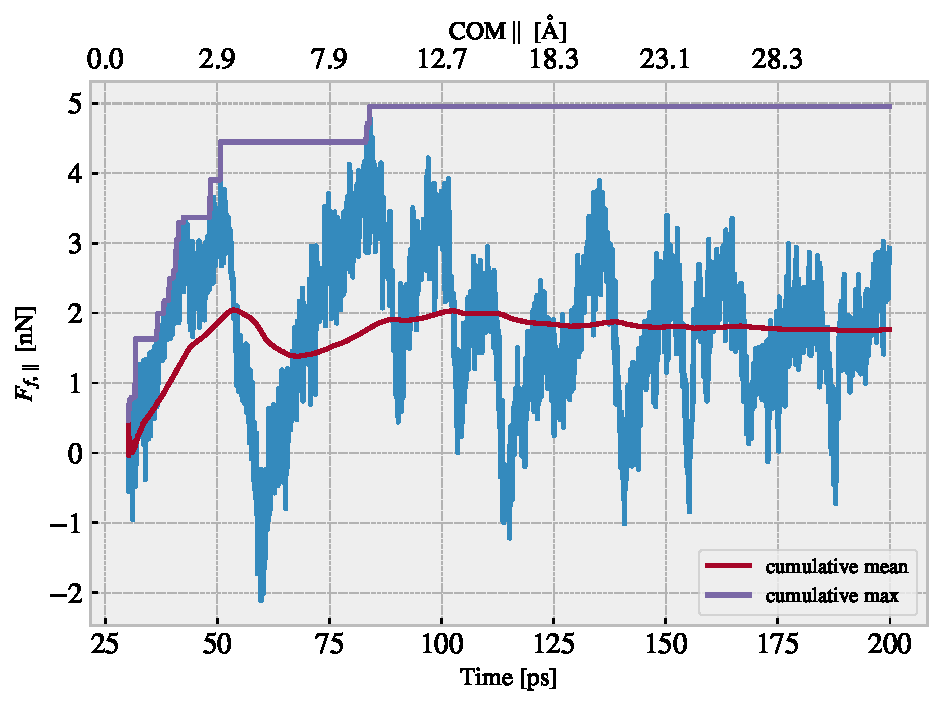
\includegraphics[width=0.7\linewidth]{figures/drag1.pdf}
		\caption{Friction force parallel to drag direction with normal force $F_N = 200$ nN. Drag distance = 40 Å}
	\end{figure}	
	
\end{frame}

\begin{frame}
	\frametitle{Stage 2 - MD measurements}
	\framesubtitle{Friction force}

	
	\begin{figure}
		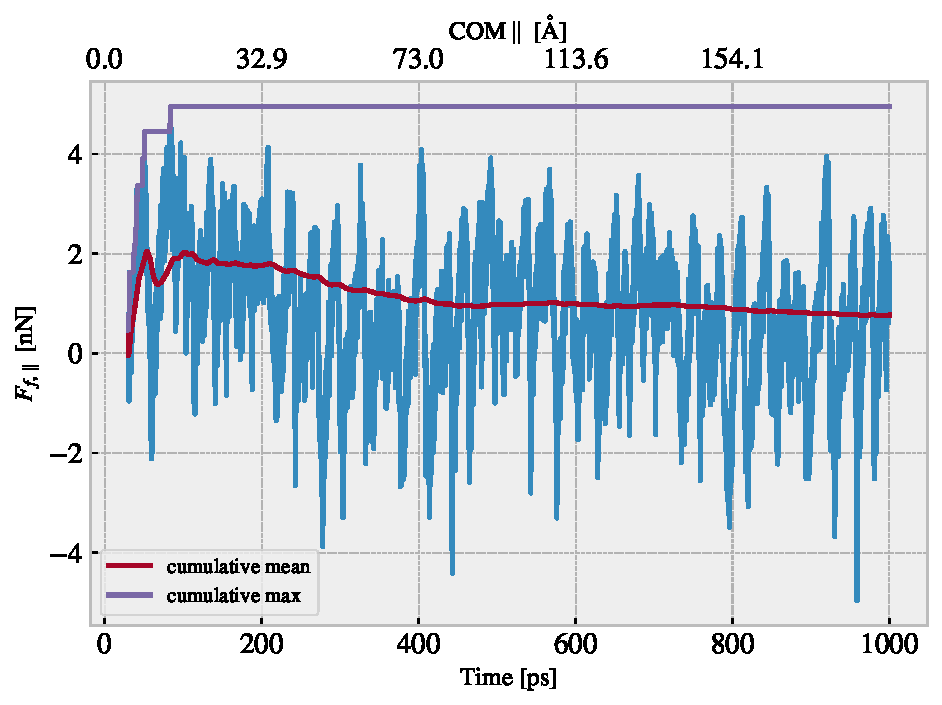
\includegraphics[width=0.7\linewidth]{figures/drag2.pdf}
		\caption{Friction force parallel to drag direction with normal force $F_N = 200$ nN. Drag distance = 200 Å.}
	\end{figure}	
	
\end{frame}



\begin{frame}
	\frametitle{Stage 2 - MD measurements}
	\framesubtitle{Contact area}

	
	\begin{figure}
		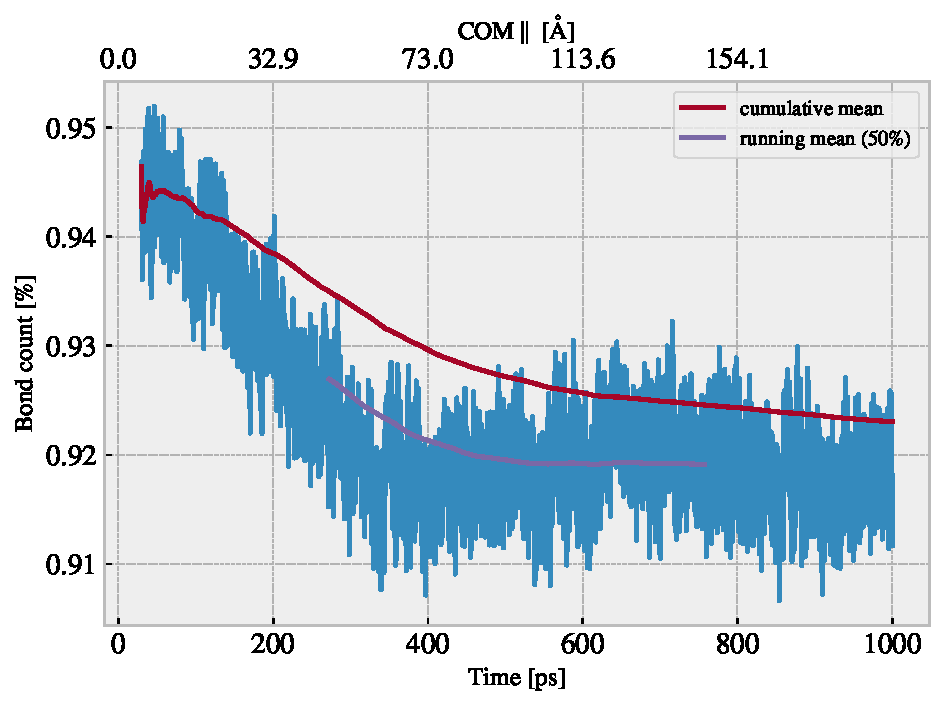
\includegraphics[width=0.7\linewidth]{figures/contact1.pdf}
		\caption{Contact bond count with normal force $F_N = 200$ nN. Drag distance = 200 Å.}
	\end{figure}	
	
\end{frame}

\begin{frame}
	\frametitle{Stage 2 - MD measurements}
	\framesubtitle{Contact area}

	
	\begin{figure}
		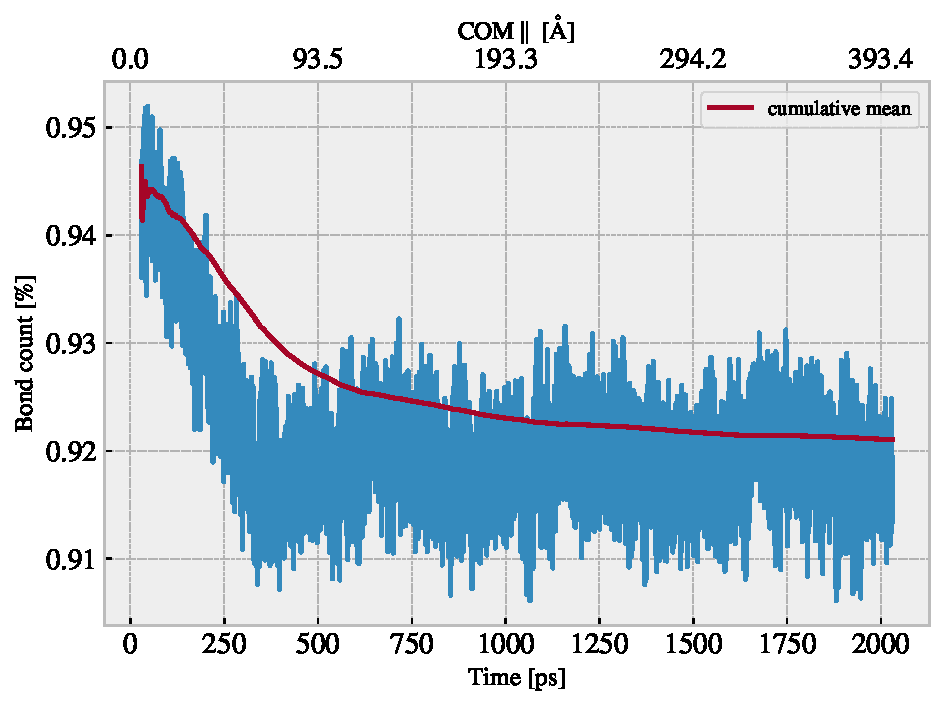
\includegraphics[width=0.7\linewidth]{figures/contact2.pdf}
		\caption{Contact bond count with normal force $F_N = 200$ nN. Drag distance = 400 Å.}
	\end{figure}	
	
\end{frame}


\begin{frame}
	\frametitle{Stage 2 - MD measurements}
	\framesubtitle{Static non-bonded regions}


	\begin{figure}
		\centering    
		\movie[open]{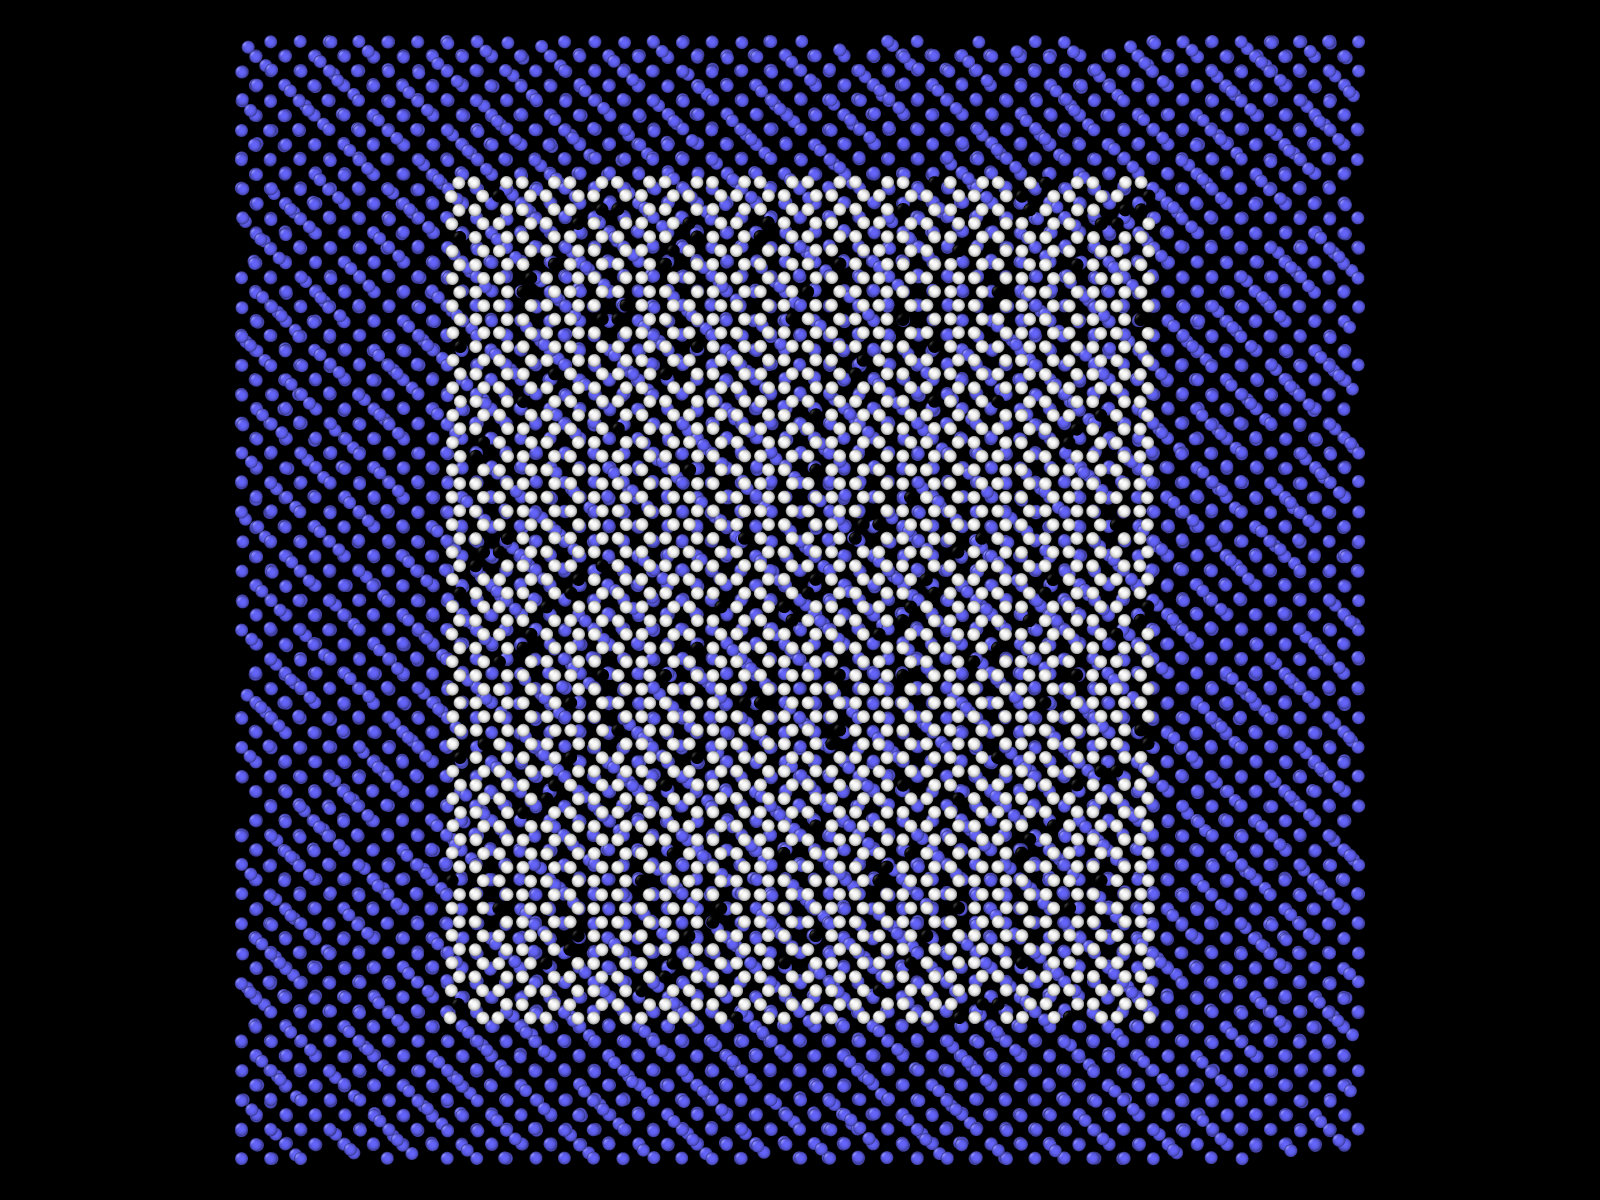
\includegraphics[width=0.95\textheight, keepaspectratio]{figures/contact_lines_notcut_nostretch.png}}{figures/contact_lines_notcut_nostretch.mov}
		\caption{Contact visualization (black atoms is non-boneded). $F_N = 200$ nN, Drag length = 400 Å.}
   \end{figure} 

\end{frame}
% \begin{frame}
% 	\frametitle{Stage 2 - MD measurements}
% 	\framesubtitle{Static non-bonded regions}


% 	\begin{figure}
% 		\centering    
% 		\movie[open]{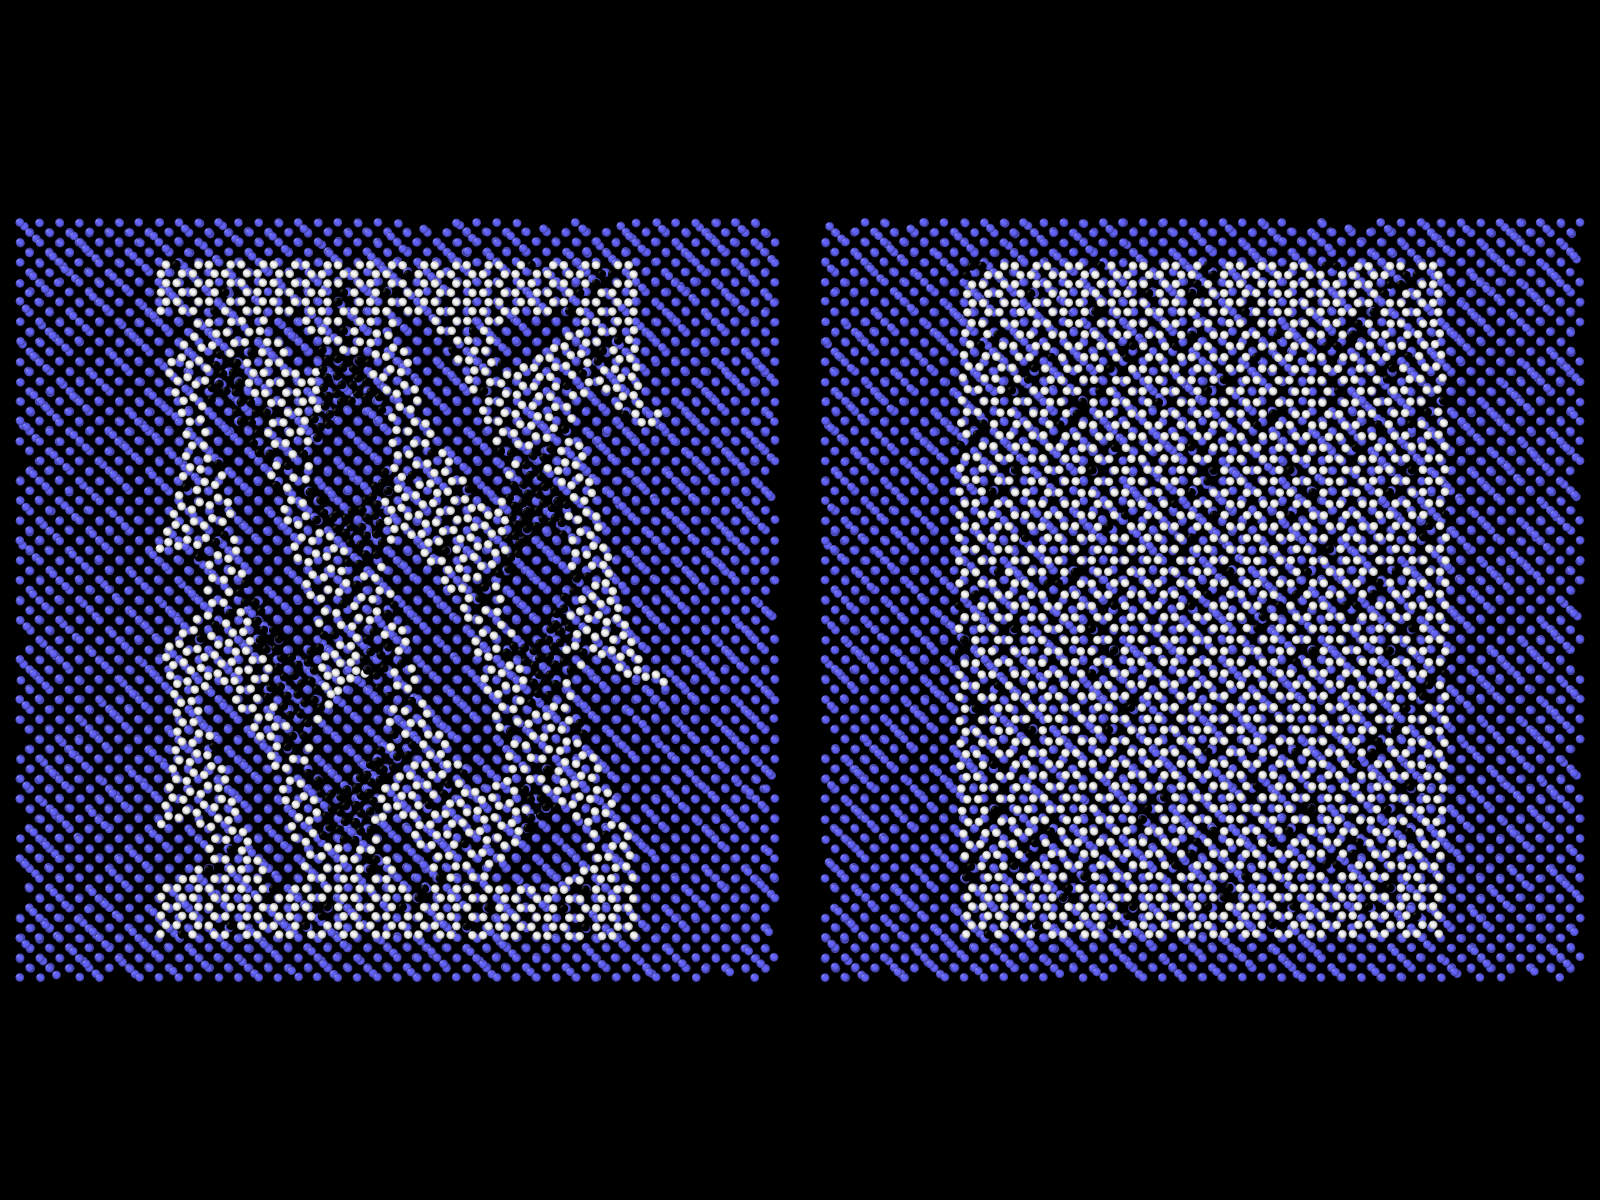
\includegraphics[width=\textheight, keepaspectratio]{figures/contact_lines_black.png}}{figures/contact_lines_black.mov}
% 		\caption{Stretch = 22 \%, $F_N = 200$ nN, Drag length = 200 Å.}
%    \end{figure} 

% \end{frame}


\begin{frame}
	\frametitle{Stage 2 - MD measurements}
	\framesubtitle{Parameters} % Optional subtitle
	
	\begin{table}
		\begin{tabular}{| l | p{35mm} | p{30mm} |} \hline
			% \toprule
			\textbf{Category} & \textbf{Parameter} & \textbf{Range} \\ \hline
			% \midrule
			Physical (free) & 
			Temperatur 		 		\newline 
			Drag speed 				&
			[0, 300] K 				\newline 
			$[1, 20]$ m/s				\\ \hline

			Physical (ML input) &
			Cut configuration 		\newline
			Scan angle 				\newline
			Stretch amount 			\newline
			Normal force 			&
			No ruptures 			\newline
			$[0, 90^{\circ}]$ 		\newline
			$[0, 20]$ \% 				\newline
			$[10, 200]$ nN 			\\ \hline

			MD settings &
			Relax and pauses \newline
			Stretch speed \newline
			Drag spring constant \newline
			Drag length \newline
			Sheet size &
			$\sim 10$ ps			\newline
			$[0.5, 0.1]$ \%/ps  	\newline
			$[10, \infty]$ N/m 		\newline
			$[50, 400]$ Å 			\newline
			$\sim 62 \times 75$ Å	\\ \hline
		\end{tabular}
		\caption{Relevant parameters of MD simulation and approximate ranges.}
	\end{table}
	
	
\end{frame}



% \begin{frame}
% 	\frametitle{Stage 2 - MD measurements}
% 	\framesubtitle{....}
% 	\begin{figure}
% 		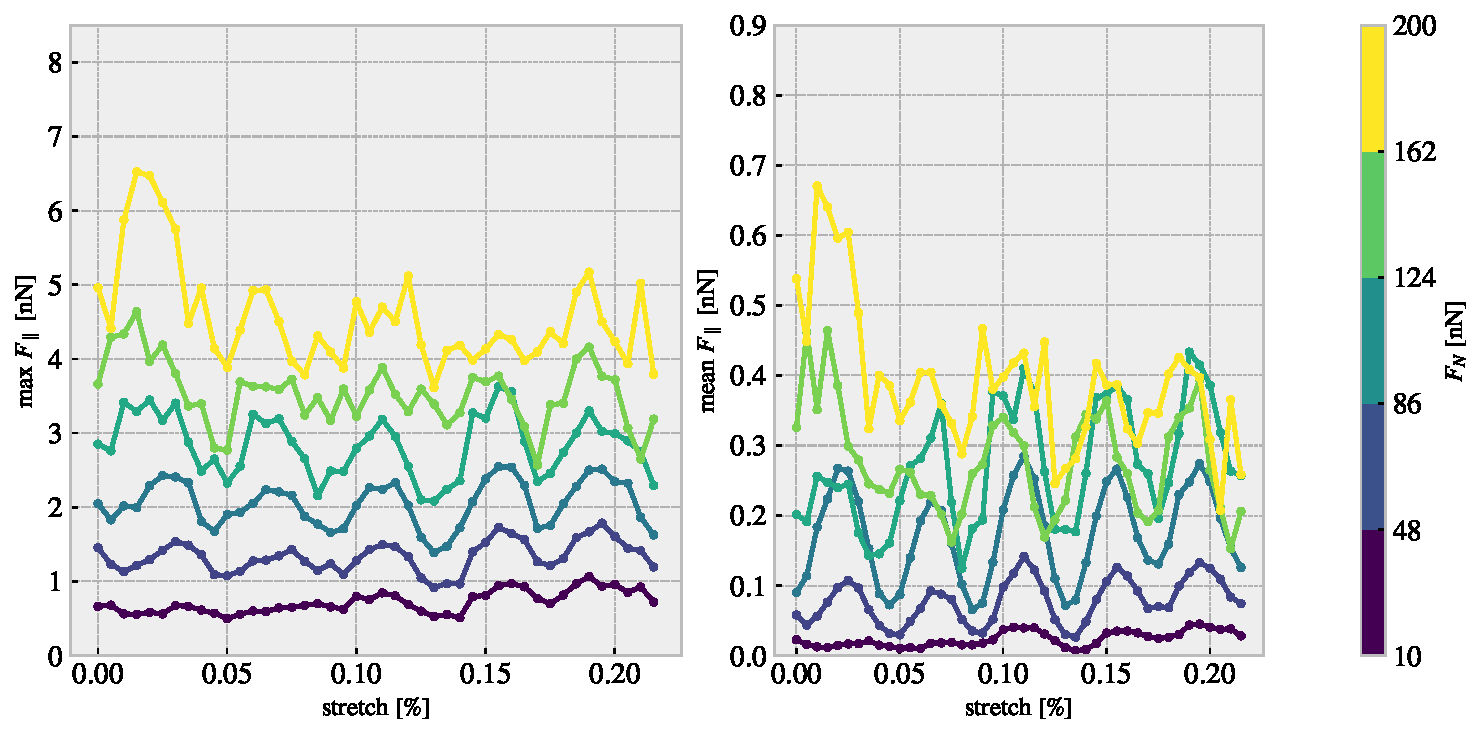
\includegraphics[width=\linewidth]{figures/multi_nocuts.pdf}
% 		\caption{(Left) Max friction force. (Right) mean friction force of the last half (50\%) of the data}
% 	\end{figure}	
	
% \end{frame}

% \begin{frame}
% 	\frametitle{Stage 2 - MD measurements}
% 	\framesubtitle{...}
% 	\begin{figure}
% 		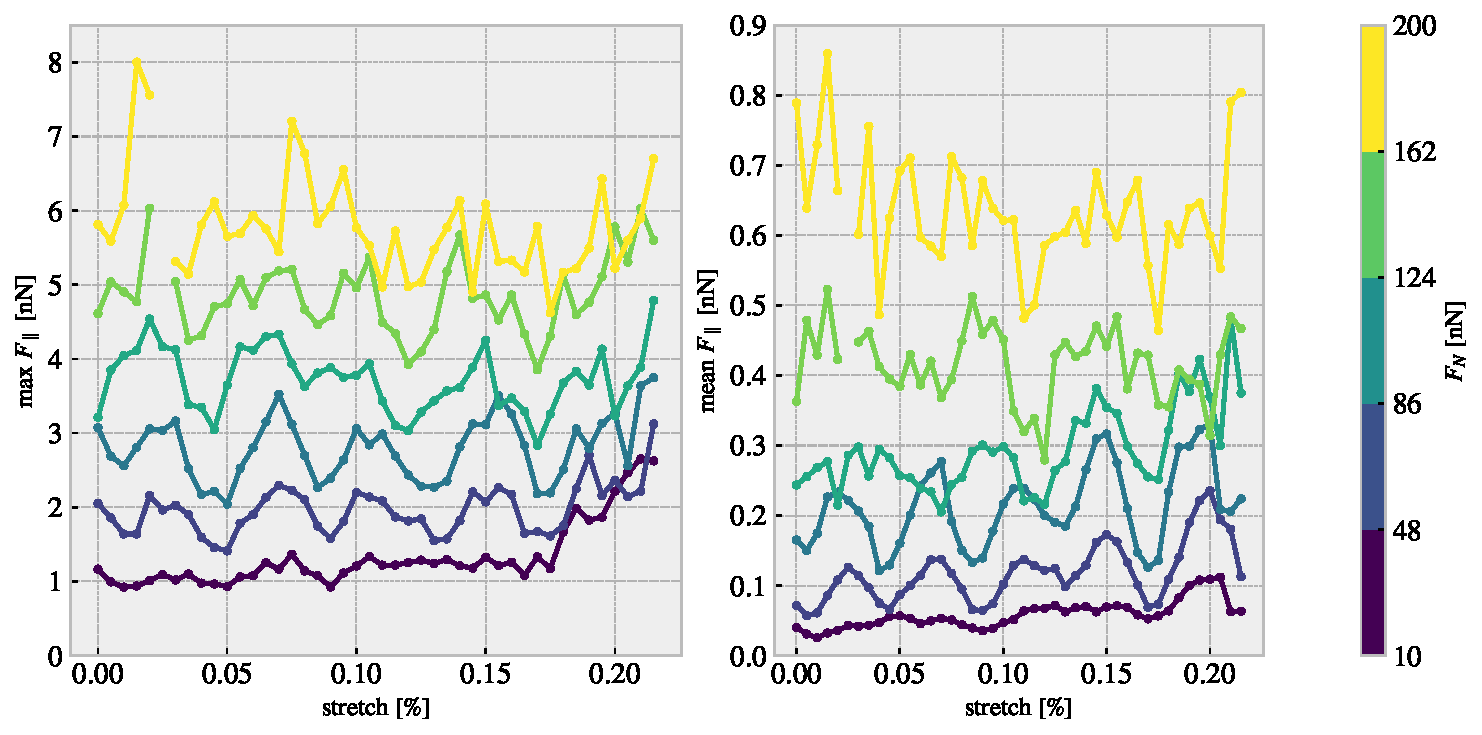
\includegraphics[width=\linewidth]{figures/multi_cuts.pdf}
% 		\caption{(Left) Max friction force. (Right) mean friction force of the last half (50\%) of the data.}
% 	\end{figure}	
	
% \end{frame}


\begin{frame}
	\frametitle{Stage 2 - MD measurements}
	\framesubtitle{Varying normal force and stretch}
	\begin{figure}
		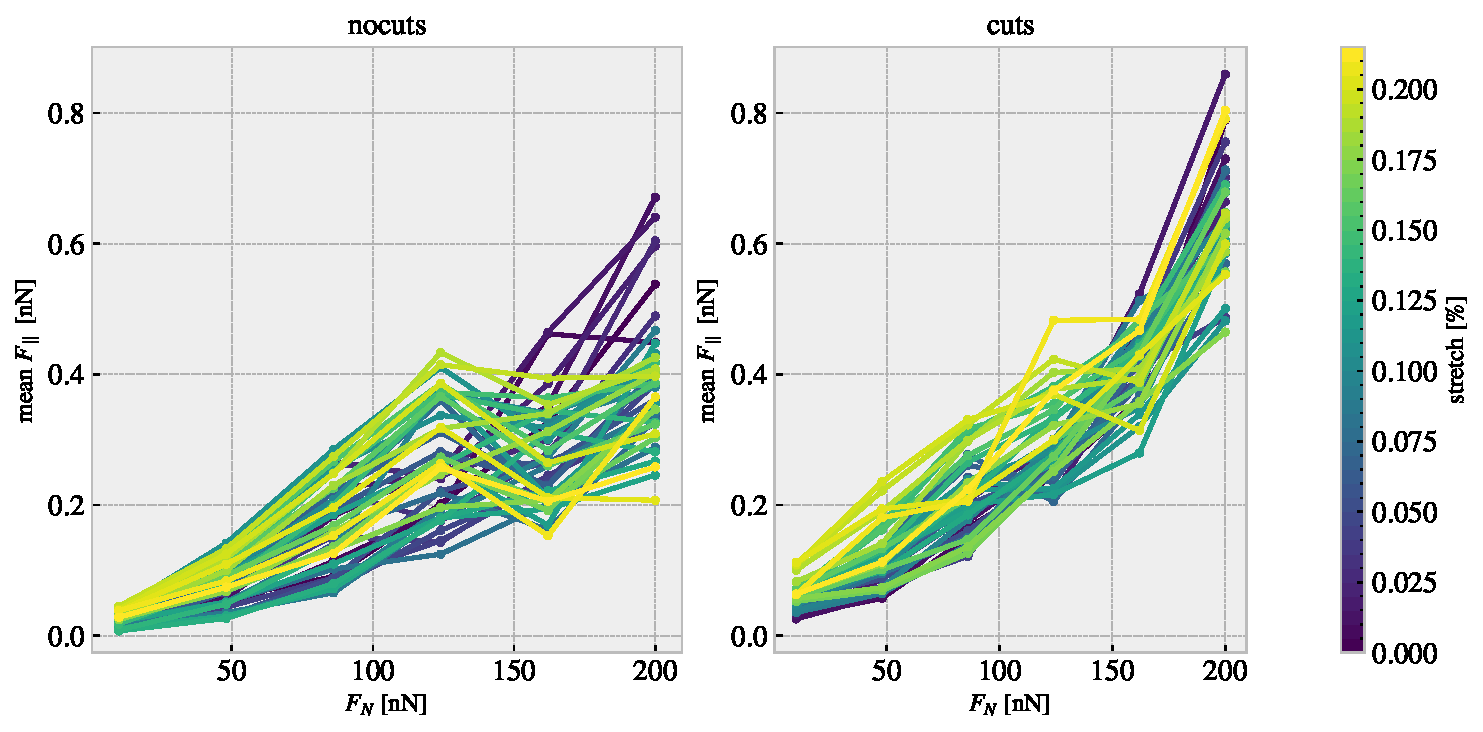
\includegraphics[width=\linewidth]{figures/multi0.pdf}
		\caption{Mean friction force $F_{\parallel}$ parallel to drag direction versus applied normal force $(F_N)$ with and without cuts.}
	\end{figure}	
\end{frame}

\begin{frame}
	\frametitle{Stage 2 - MD measurements}
	\framesubtitle{Varying normal force and stretch}
	\begin{figure}
		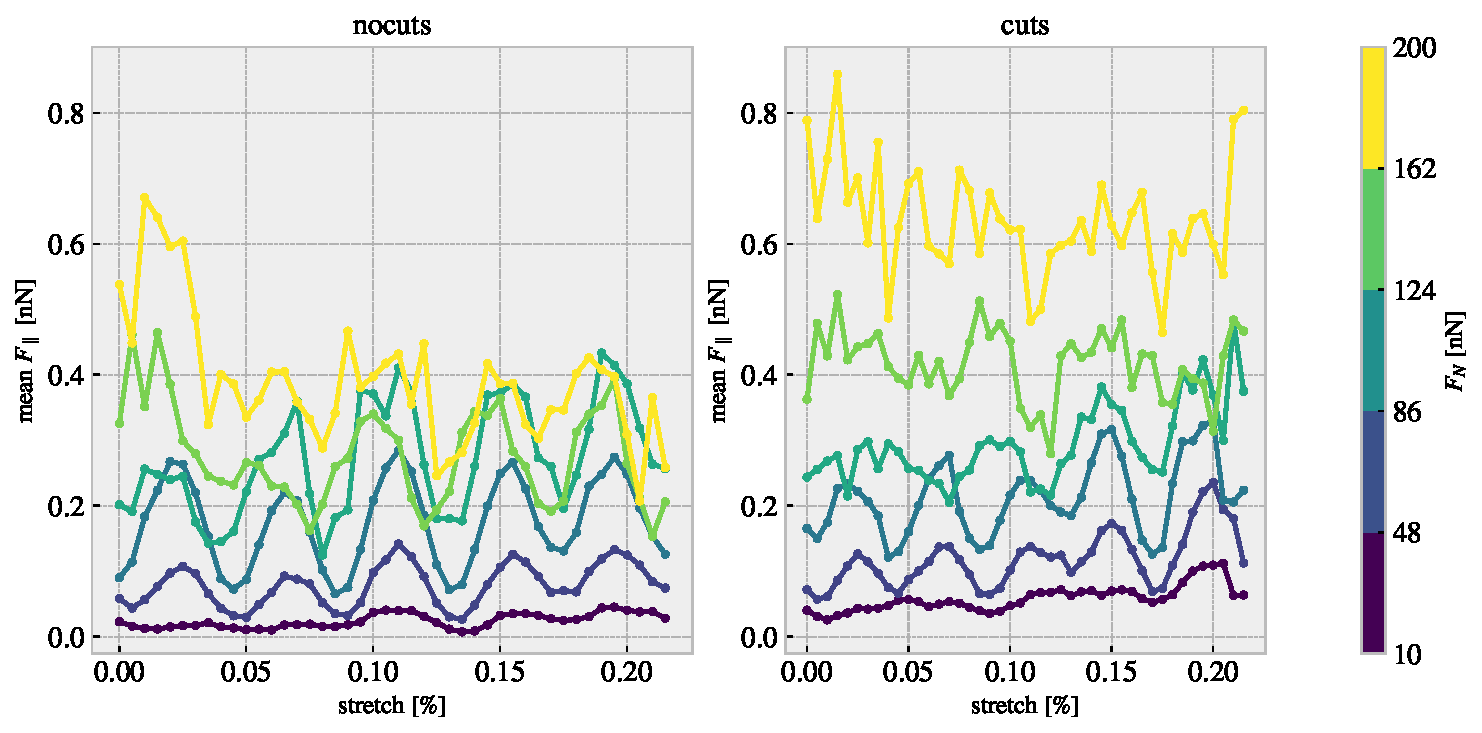
\includegraphics[width=\linewidth]{figures/multi2.pdf}
		\caption{Mean friction force $F_{\parallel}$ parallel to drag direction versus stretch of the sheet with and without cuts.}
	\end{figure}	
\end{frame}

\begin{frame}
	\frametitle{Stage 2 - MD measurements}
	\framesubtitle{Varying normal force and stretch}
	\begin{figure}
		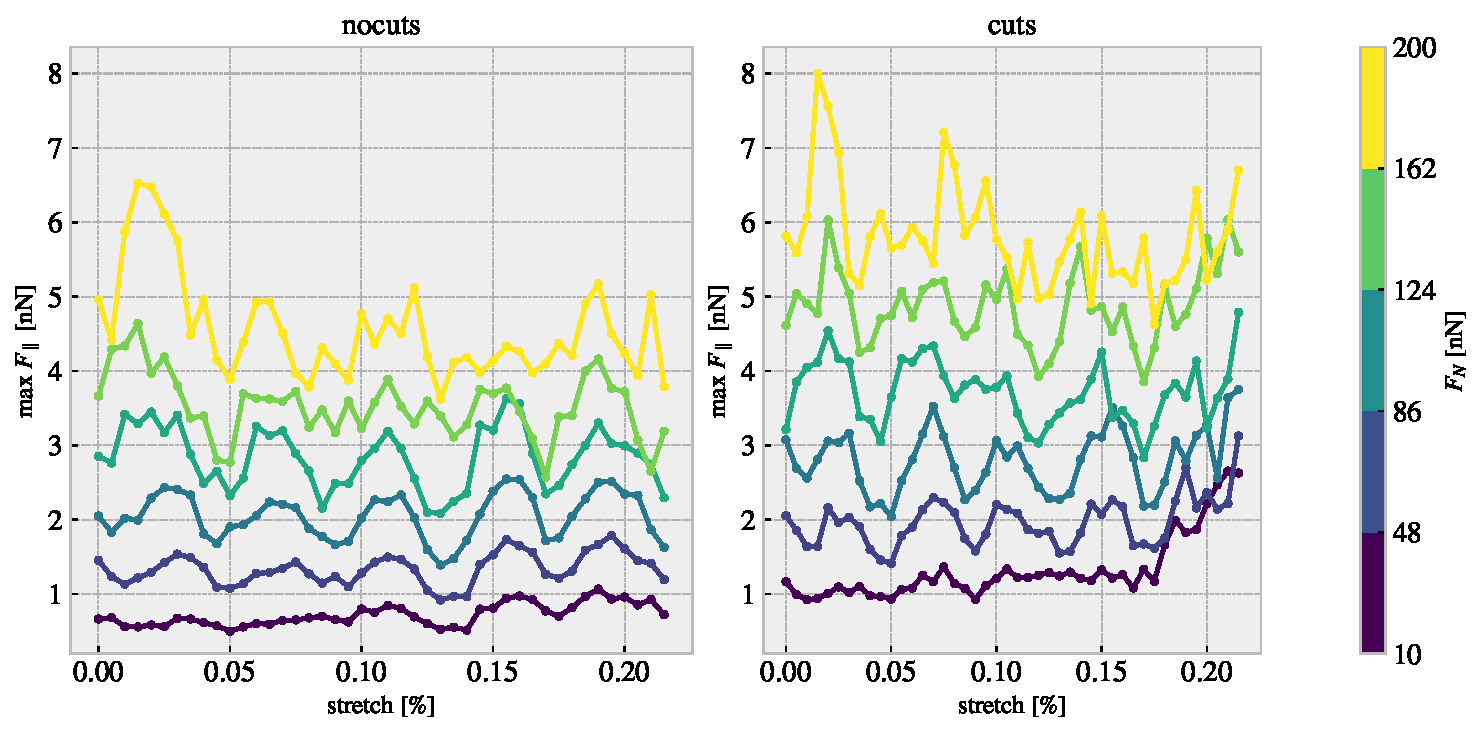
\includegraphics[width=\linewidth]{figures/multi1.pdf}
		\caption{Max friction force $F_{\parallel}$ parallel to drag direction versus stretch of the sheet with and without cuts.}
	\end{figure}	
\end{frame}


\begin{frame}
	\frametitle{Stage 2 - MD measurements}
	\framesubtitle{Varying normal force and stretch}
	\begin{figure}
		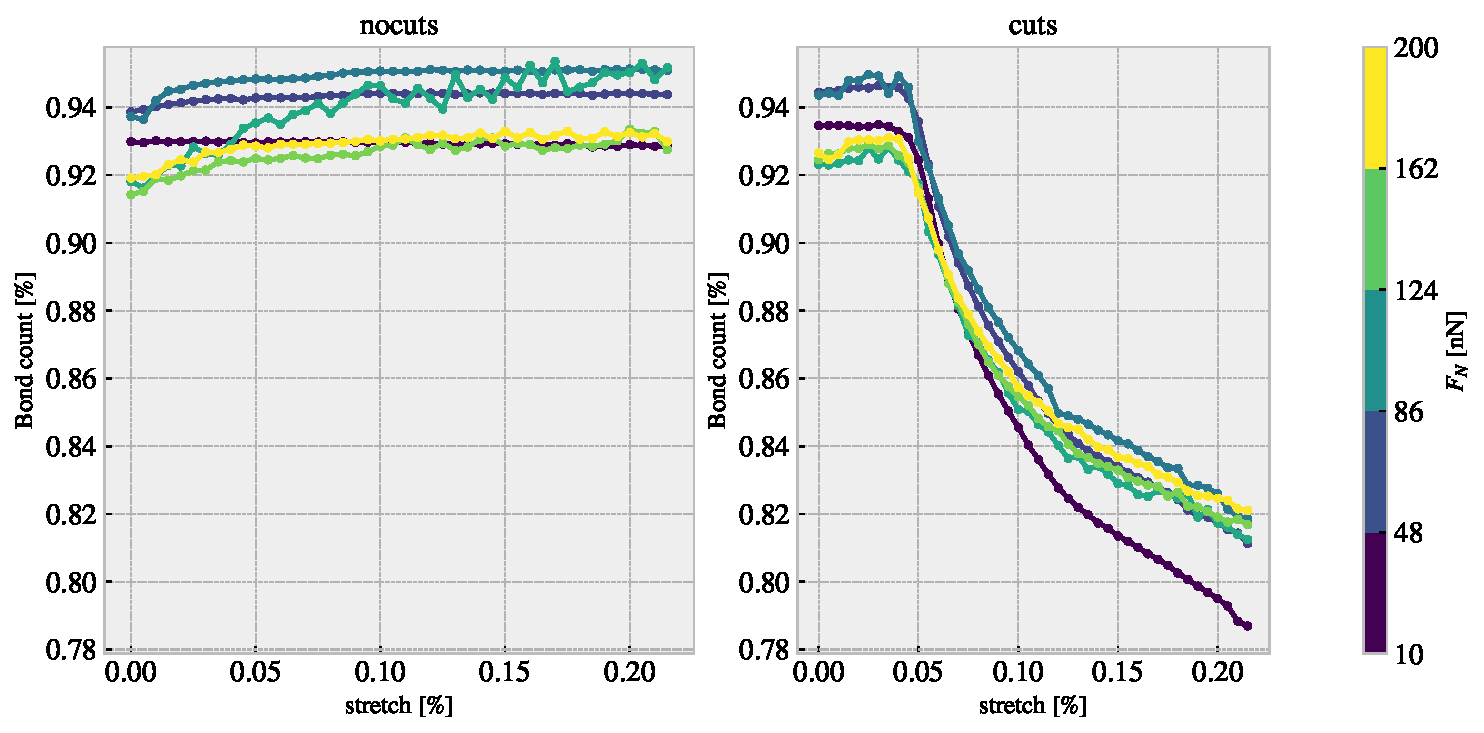
\includegraphics[width=\linewidth]{figures/multi3.pdf}
		\caption{Contact bonds versus stretch of the sheet with and without cuts.}
	\end{figure}	
\end{frame}

\begin{frame}
	\frametitle{Stage 2 - MD measurements}
	\framesubtitle{Varying normal force and stretch}
	\begin{figure}
		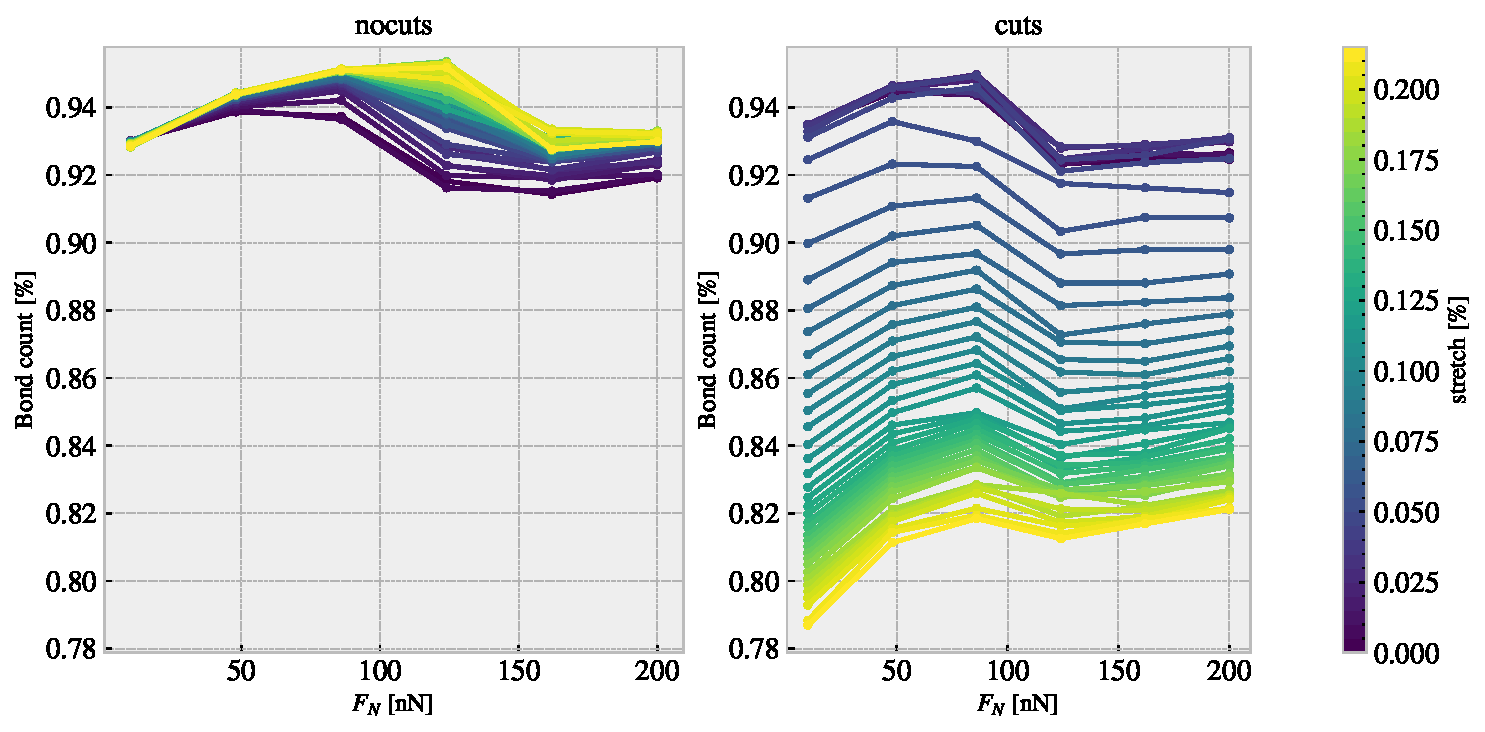
\includegraphics[width=\linewidth]{figures/multi4.pdf}
		\caption{Contact bonds versus normal force $F_N$ of the sheet with and without cuts.}
	\end{figure}	
\end{frame}

\begin{frame}
	\frametitle{Stage 2 - MD measurements}
	\framesubtitle{Varying normal force and stretch}
	\begin{figure}
		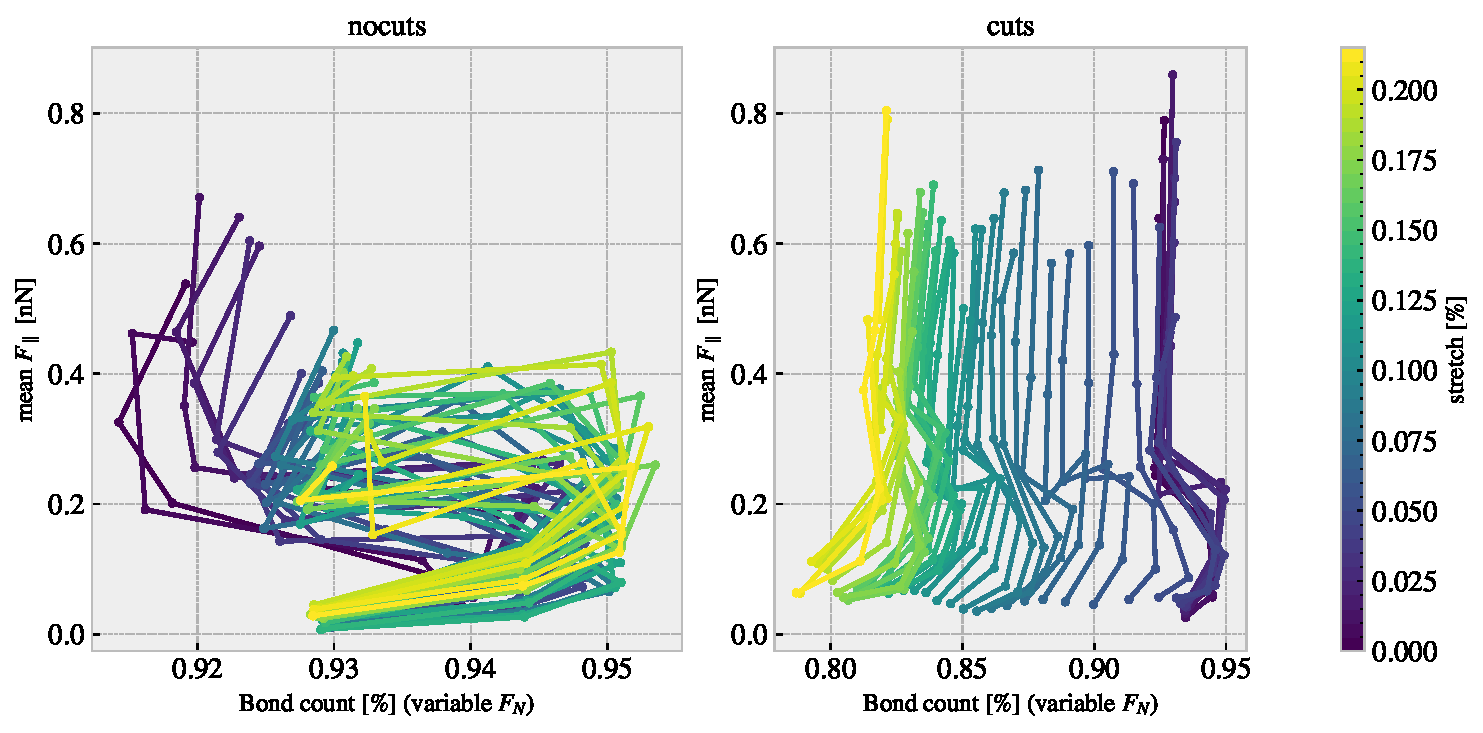
\includegraphics[width=\linewidth]{figures/multi5.pdf}
		\caption{Mean friction force $F_{\parallel}$ parallel to drag direction versus contact bonds (varied by normal force $F_N$) with and without cuts.}
	\end{figure}	
\end{frame}

\begin{frame}
	\frametitle{Stage 2 - MD measurements}
	\framesubtitle{Varying normal force and stretch}
	\begin{figure}
		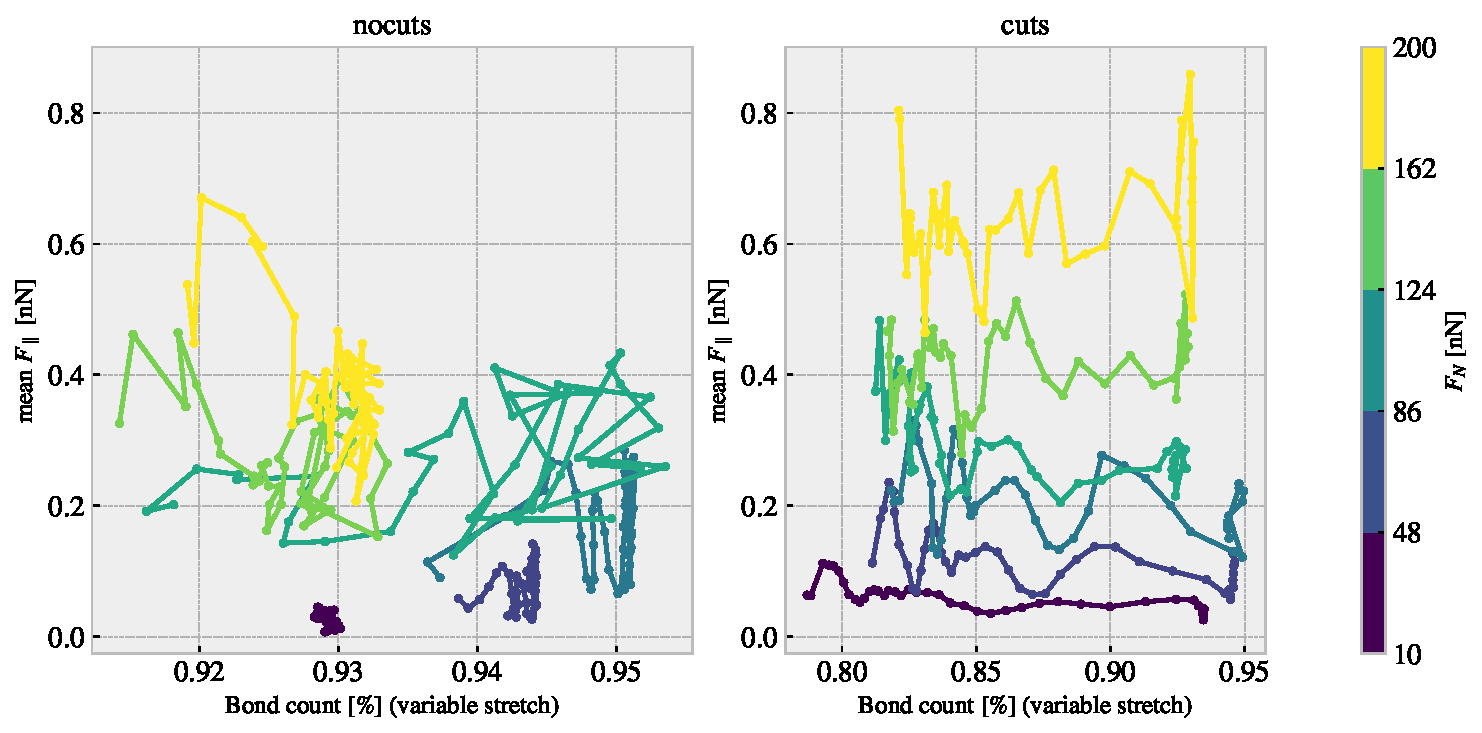
\includegraphics[width=\linewidth]{figures/multi6.pdf}
		\caption{Mean friction force $F_{\parallel}$ parallel to drag direction versus contact bonds (varied by normal force stretch) with and without cuts.}
	\end{figure}	
\end{frame}




\begin{frame}
	\frametitle{Stage 2 - MD measurements}
	\framesubtitle{New data}

	{\Large New data} 
	\newline

	Invistigate different $F_N$ range:
	\begin{align*}
		F_N = [10, 200] \rightarrow [0.1, 1] \text{nN} 
	\end{align*}

\end{frame}

% Low FN



\begin{frame}
	\frametitle{Stage 2 - MD measurements}
	\framesubtitle{Varying normal force and stretch}
	\begin{figure}
		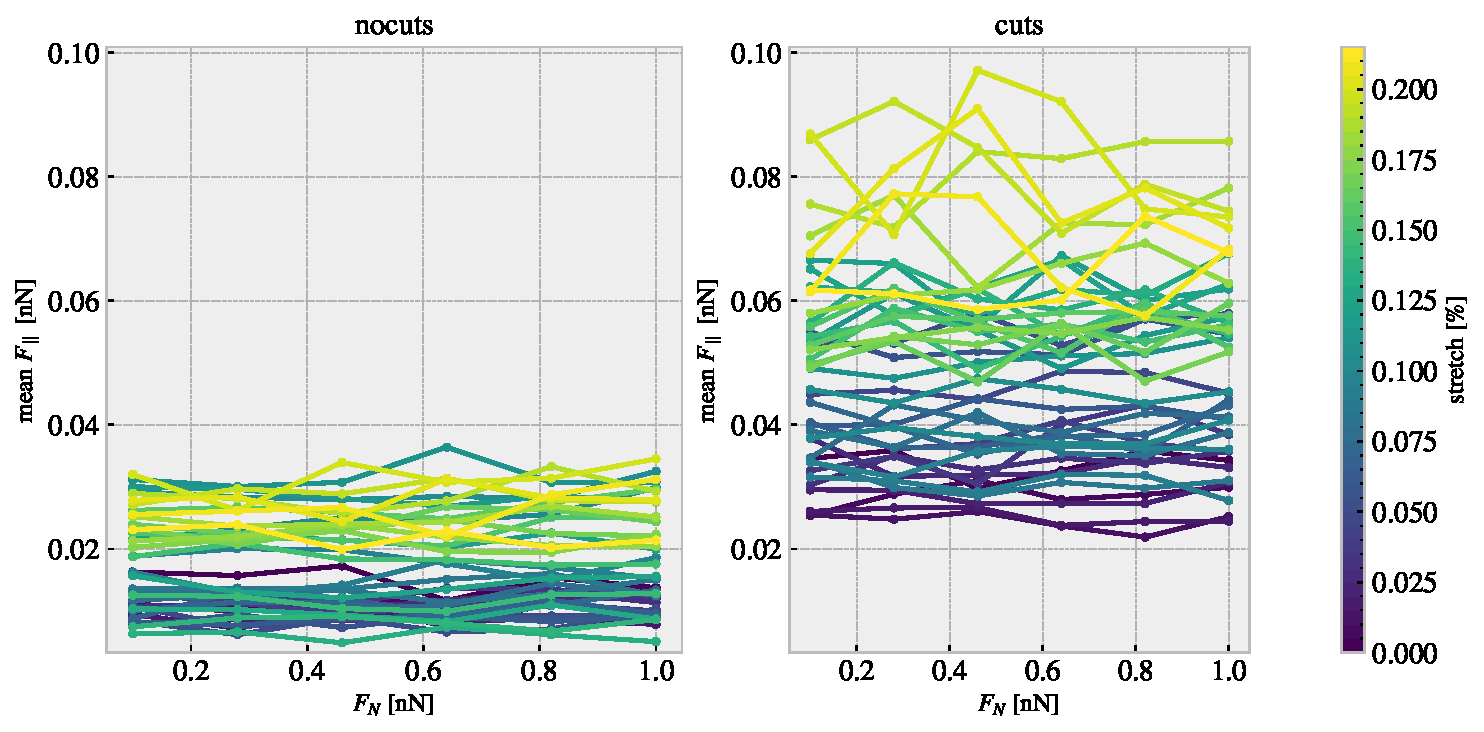
\includegraphics[width=\linewidth]{figures/multi_lowFN0.pdf}
		\caption{Mean friction force $F_{\parallel}$ parallel to drag direction versus applied normal force $(F_N)$ with and without cuts.}
	\end{figure}	
\end{frame}

\begin{frame}
	\frametitle{Stage 2 - MD measurements}
	\framesubtitle{Varying normal force and stretch}
	\begin{figure}
		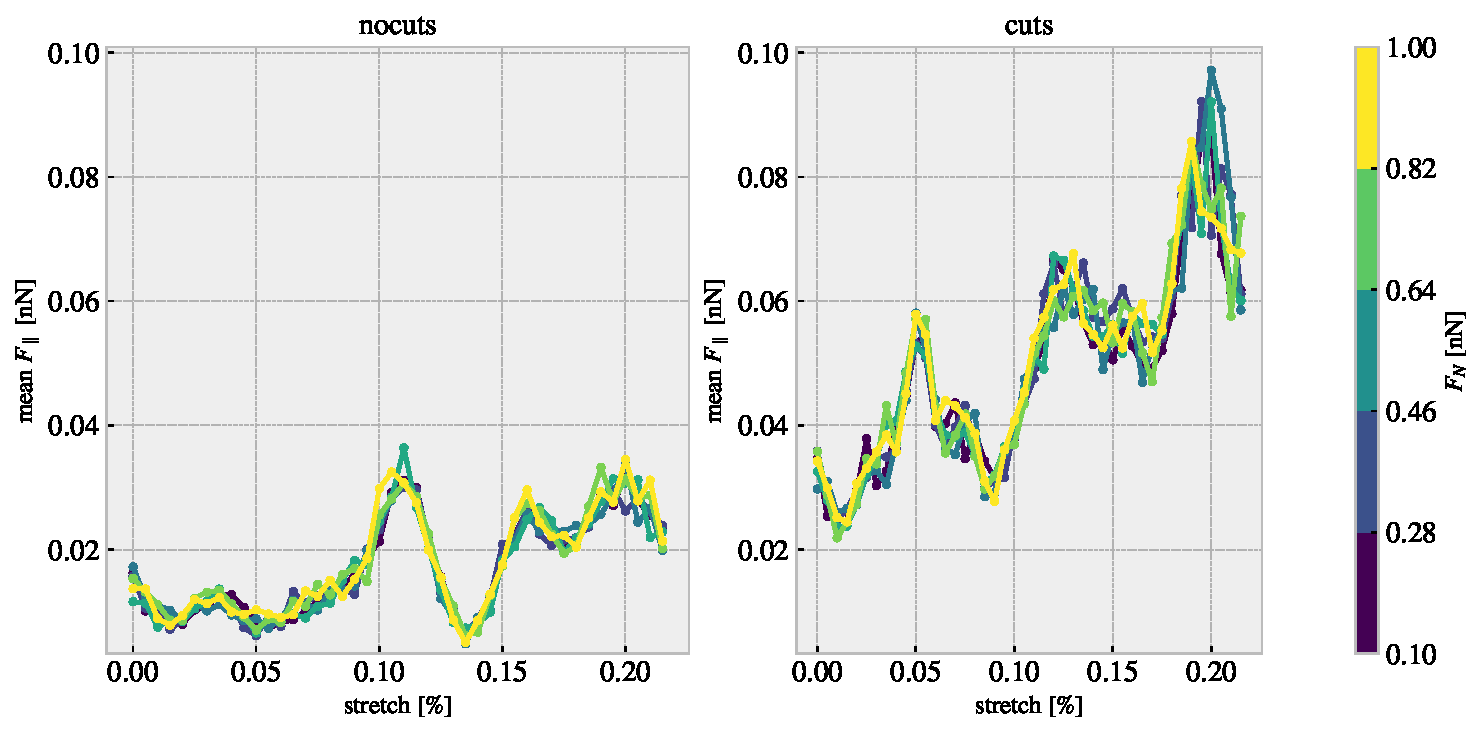
\includegraphics[width=\linewidth]{figures/multi_lowFN2.pdf}
		\caption{Mean friction force $F_{\parallel}$ parallel to drag direction versus stretch of the sheet with and without cuts.}
	\end{figure}	
\end{frame}


\begin{frame}
	\frametitle{Stage 2 - MD measurements}
	\framesubtitle{Varying normal force and stretch}
	\begin{figure}
		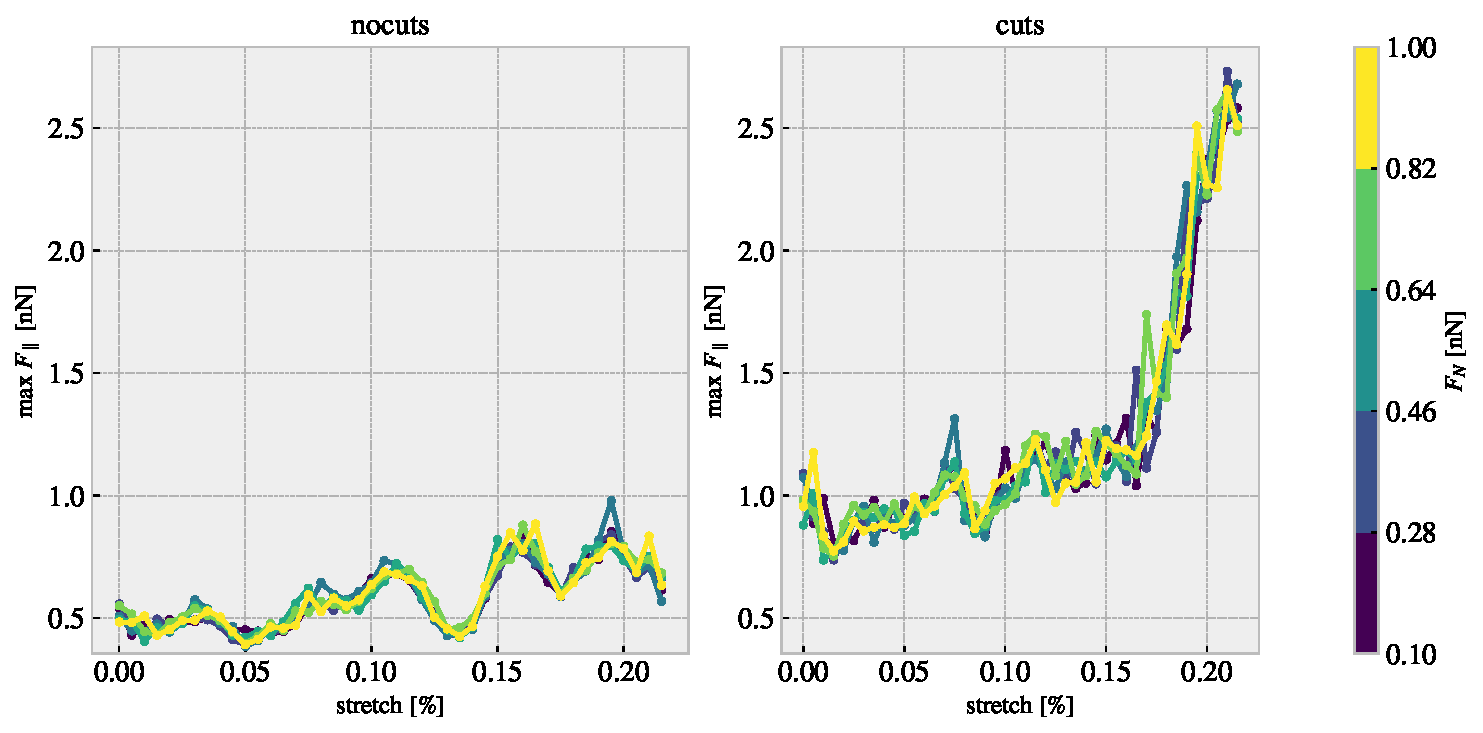
\includegraphics[width=\linewidth]{figures/multi_lowFN1.pdf}
		\caption{Max friction force $F_{\parallel}$ parallel to drag direction versus stretch of the sheet with and without cuts.}
	\end{figure}	
\end{frame}


\begin{frame}
	\frametitle{Stage 2 - MD measurements}
	\framesubtitle{Varying normal force and stretch}
	\begin{figure}
		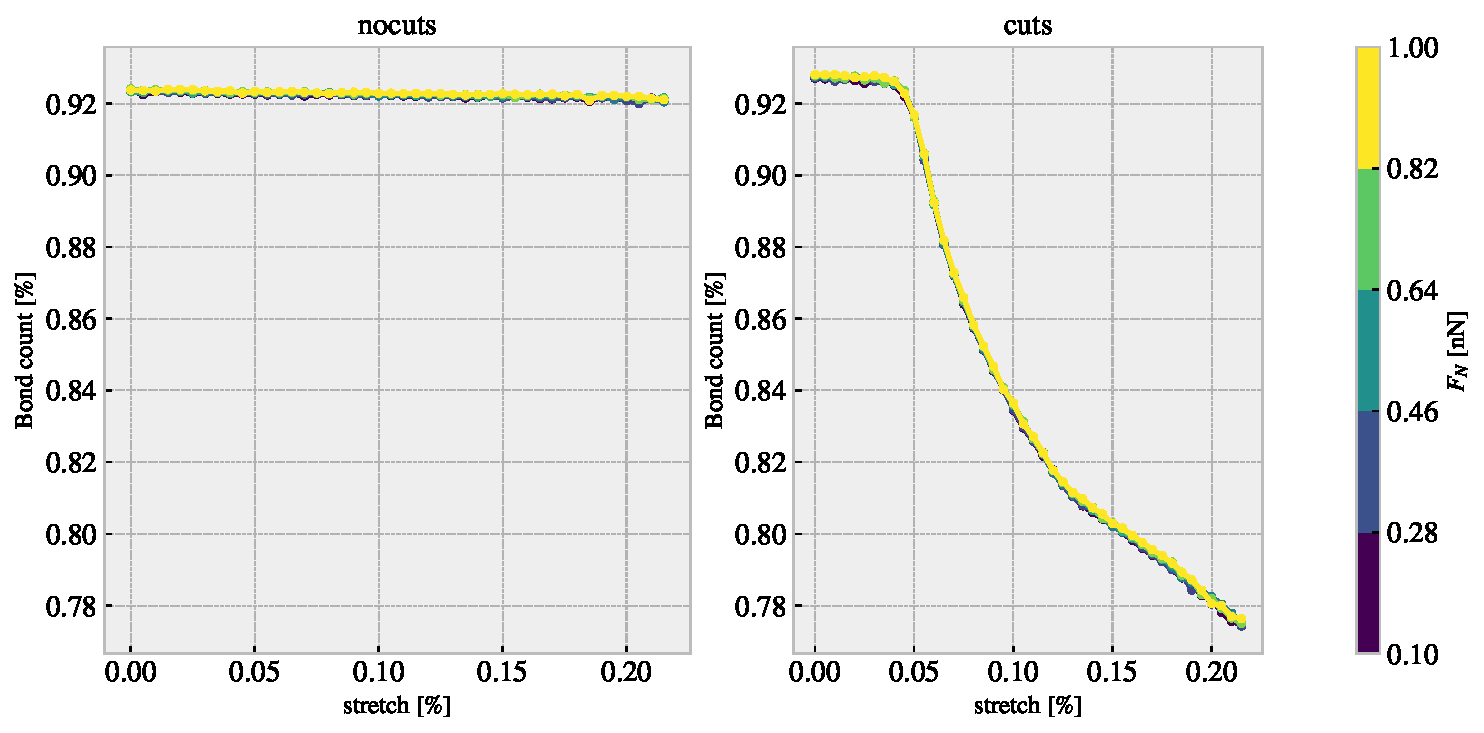
\includegraphics[width=\linewidth]{figures/multi_lowFN3.pdf}
		\caption{Contact bonds versus stretch of the sheet with and without cuts.}
	\end{figure}	
\end{frame}

\begin{frame}
	\frametitle{Stage 2 - MD measurements}
	\framesubtitle{Varying normal force and stretch}
	\begin{figure}
		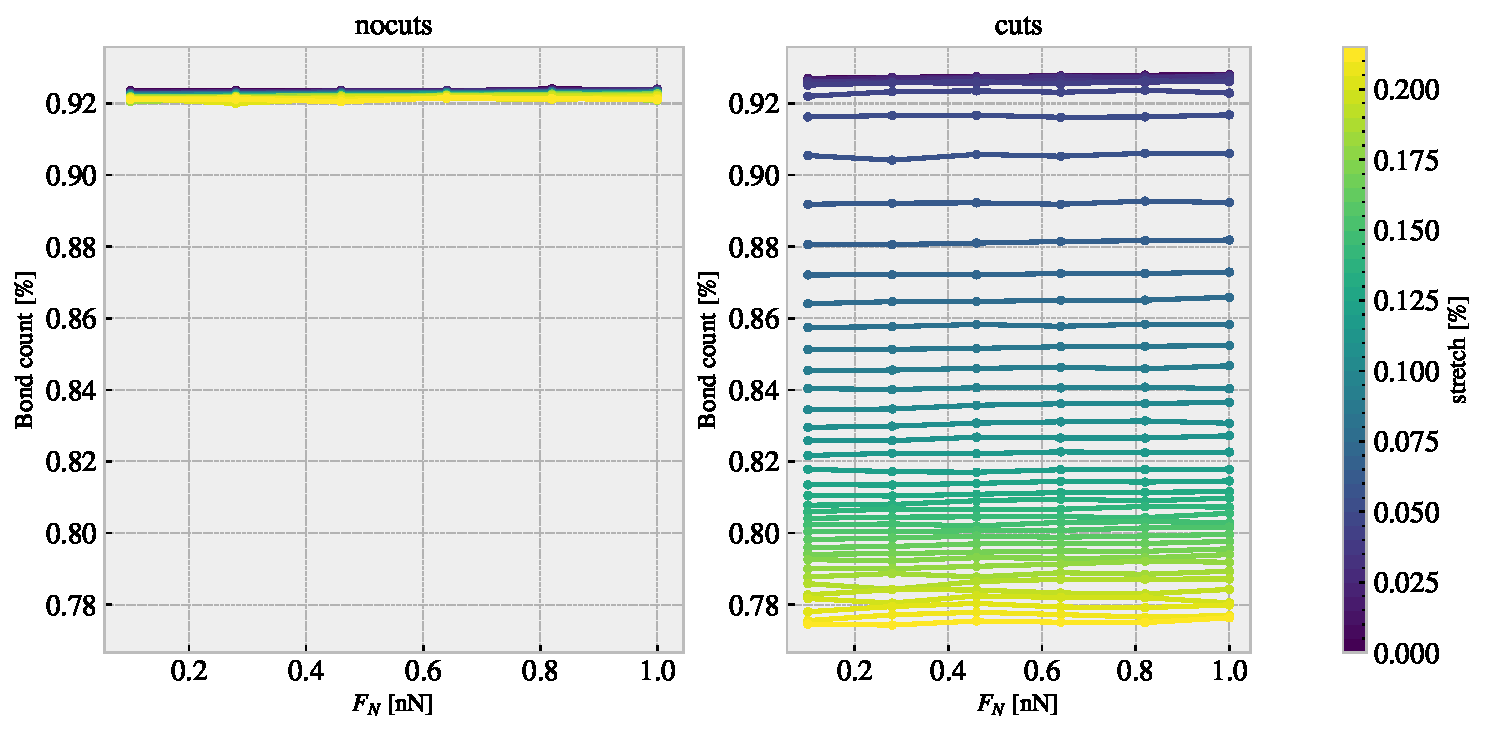
\includegraphics[width=\linewidth]{figures/multi_lowFN4.pdf}
		\caption{Contact bonds versus normal force $F_N$ of the sheet with and without cuts.}
	\end{figure}	
\end{frame}

\begin{frame}
	\frametitle{Stage 2 - MD measurements}
	\framesubtitle{Varying normal force and stretch}
	\begin{figure}
		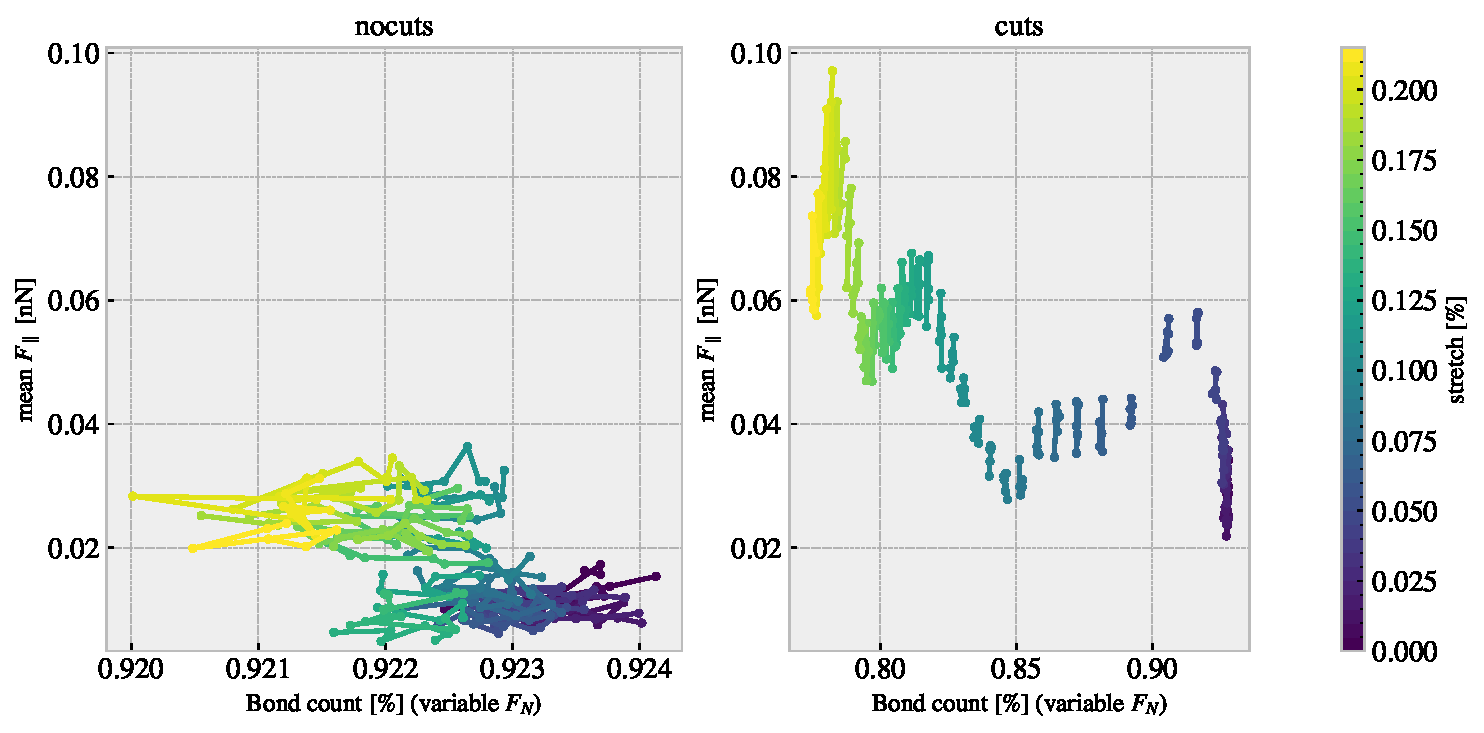
\includegraphics[width=\linewidth]{figures/multi_lowFN5.pdf}
		\caption{Mean friction force $F_{\parallel}$ parallel to drag direction versus contact bonds (varied by normal force $F_N$) with and without cuts.}
	\end{figure}	
\end{frame}

\begin{frame}
	\frametitle{Stage 2 - MD measurements}
	\framesubtitle{Varying normal force and stretch}
	\begin{figure}
		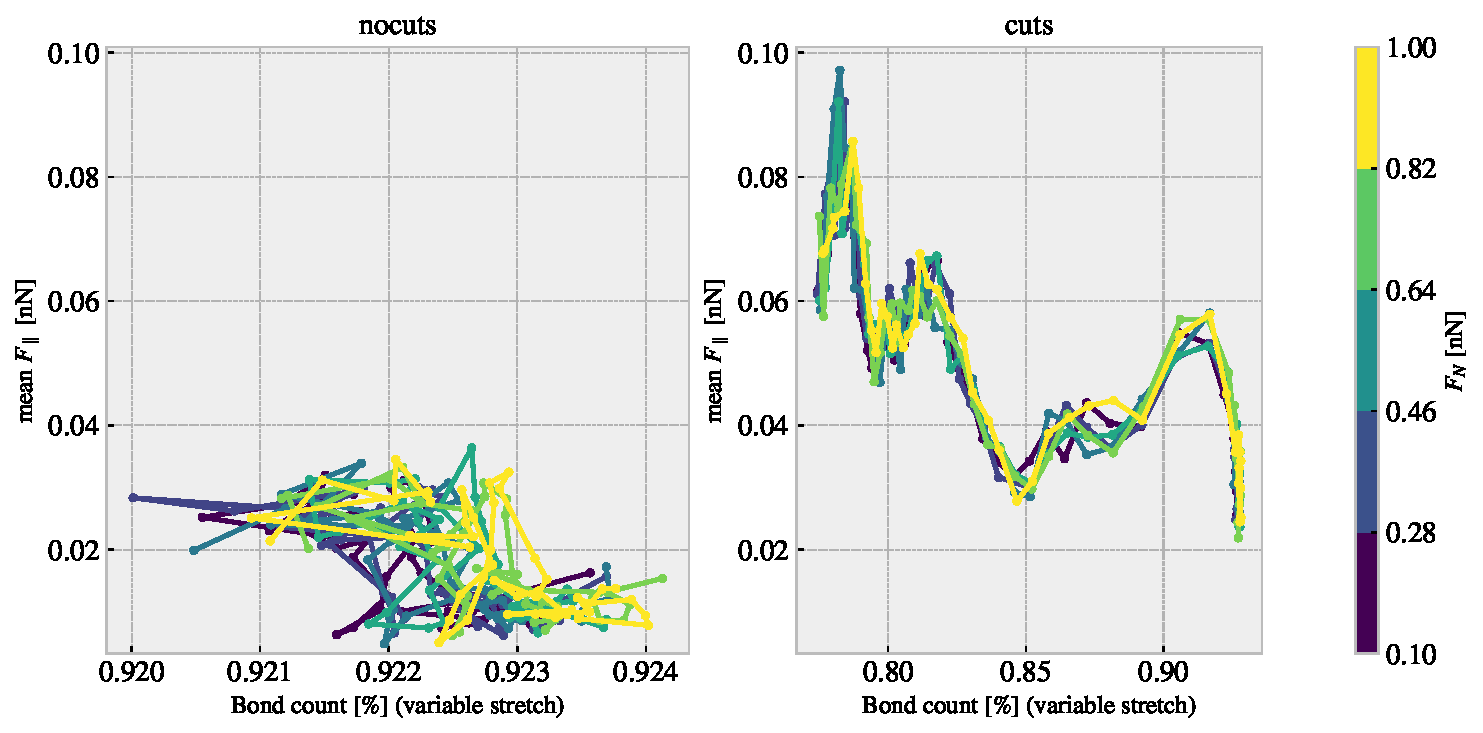
\includegraphics[width=\linewidth]{figures/multi_lowFN6.pdf}
		\caption{Mean friction force $F_{\parallel}$ parallel to drag direction versus contact bonds (varied by normal force stretch) with and without cuts.}
	\end{figure}	
\end{frame}



\begin{frame}
	\frametitle{Stage 2 - MD measurements}
	\framesubtitle{More data}

	Three different normal force ranges 
	\begin{align*}
		F_N &= [0.1, 1]\ \text{nN} \\
		F_N &= [1, 10]\ \text{nN} \\
		F_N &= [10, 86]\ \text{nN}
	\end{align*}

\end{frame}


\begin{frame}
	\frametitle{Stage 2 - MD measurements}
	\framesubtitle{Different normal force domains}
	\begin{figure}
		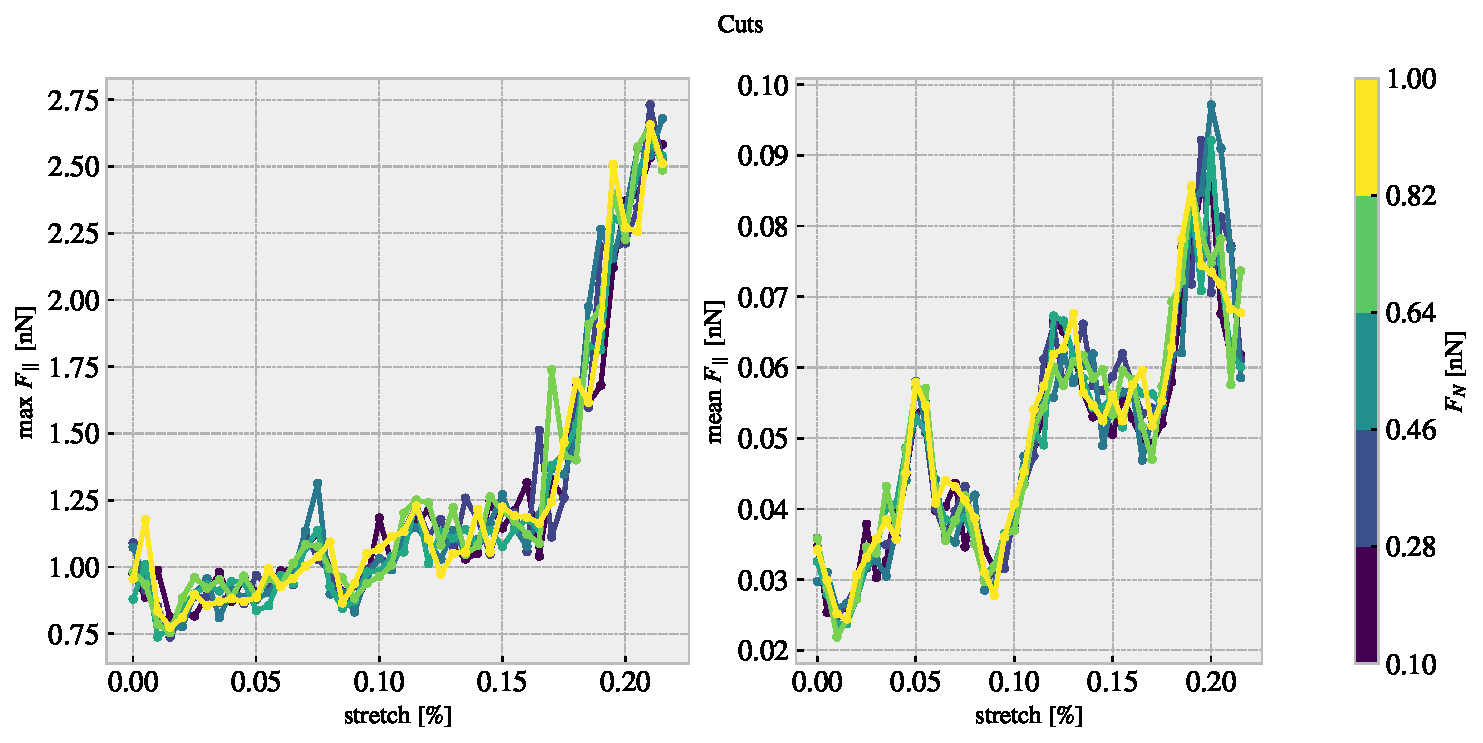
\includegraphics[width=\linewidth]{figures/max_mean_lowFN.pdf}
		\caption{Max and mean friction for $F_N = [0.1, 1]$ nN for cutted sheet}
	\end{figure}	
\end{frame}

\begin{frame}
	\frametitle{Stage 2 - MD measurements}
	\framesubtitle{Different normal force domains}
	\begin{figure}
		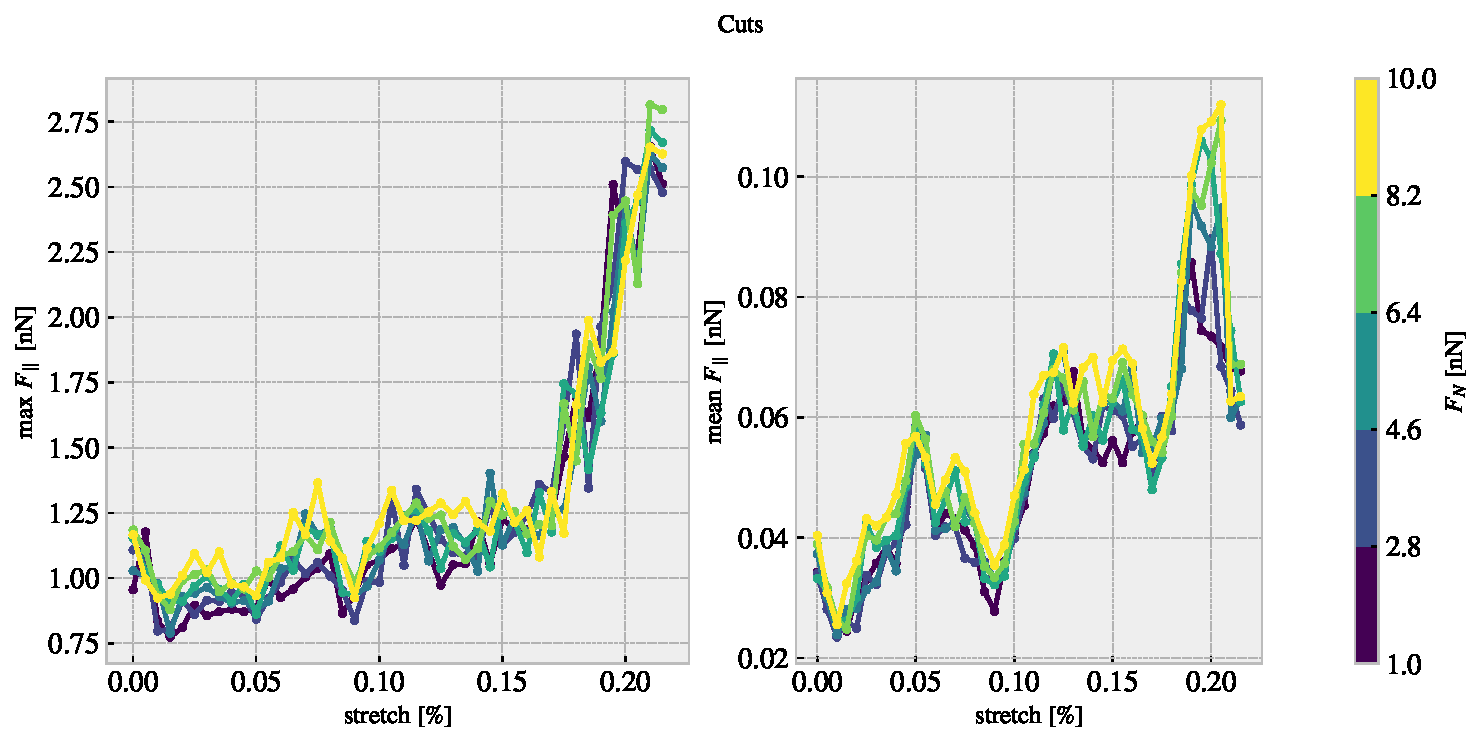
\includegraphics[width=\linewidth]{figures/max_mean_medFN.pdf}
		\caption{Max and mean friction for $F_N = [1, 10]$ nN for cutted sheet}
	\end{figure}	
\end{frame}

\begin{frame}
	\frametitle{Stage 2 - MD measurements}
	\framesubtitle{Different normal force domains}
	\begin{figure}
		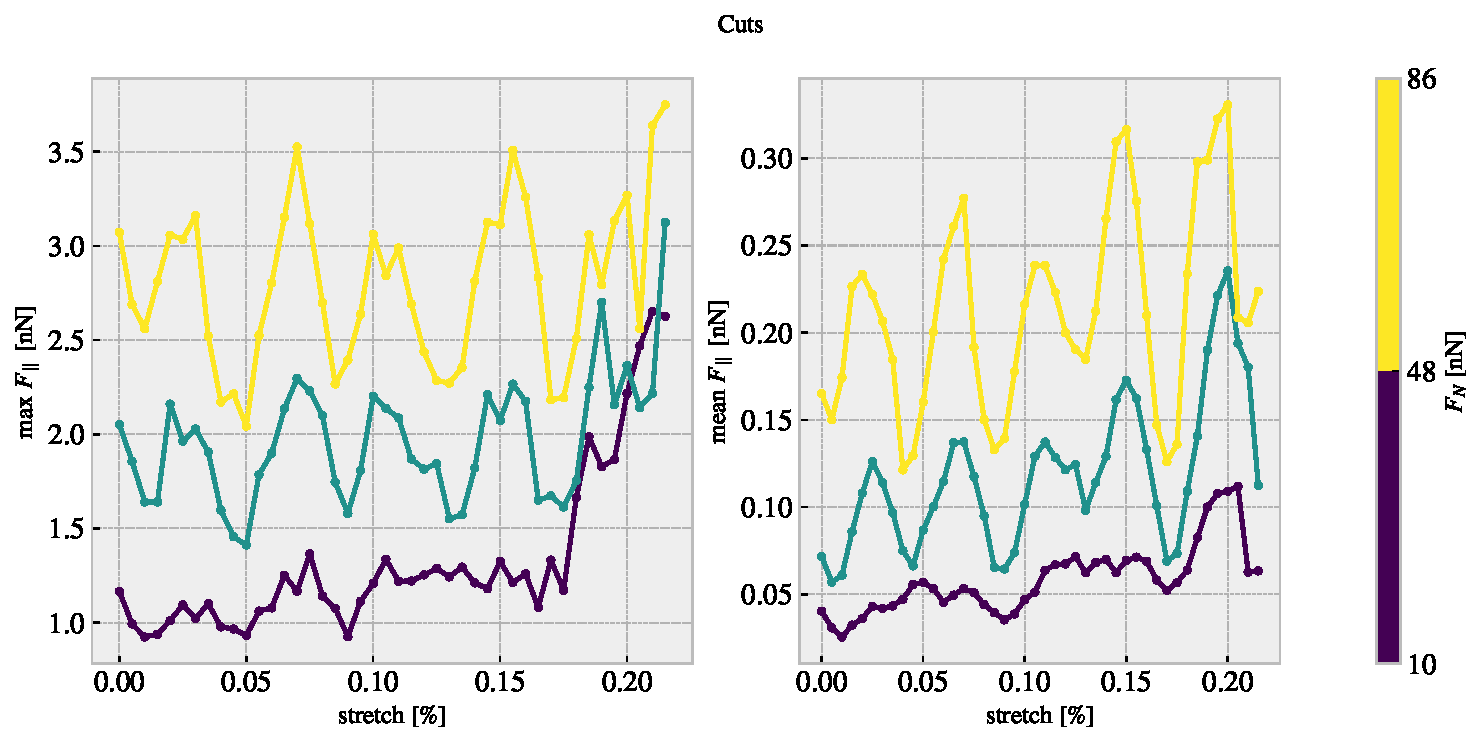
\includegraphics[width=\linewidth]{figures/max_mean_highFN.pdf}
		\caption{Max and mean friction for $F_N = [10, 86]$ nN for cutted sheet}
	\end{figure}	
\end{frame}


\begin{frame}
	\frametitle{Stage 2 - MD measurements}
	\framesubtitle{More data}

	Contribution from different parts, Full sheet = sheet + Pull blocks
	\begin{figure}
		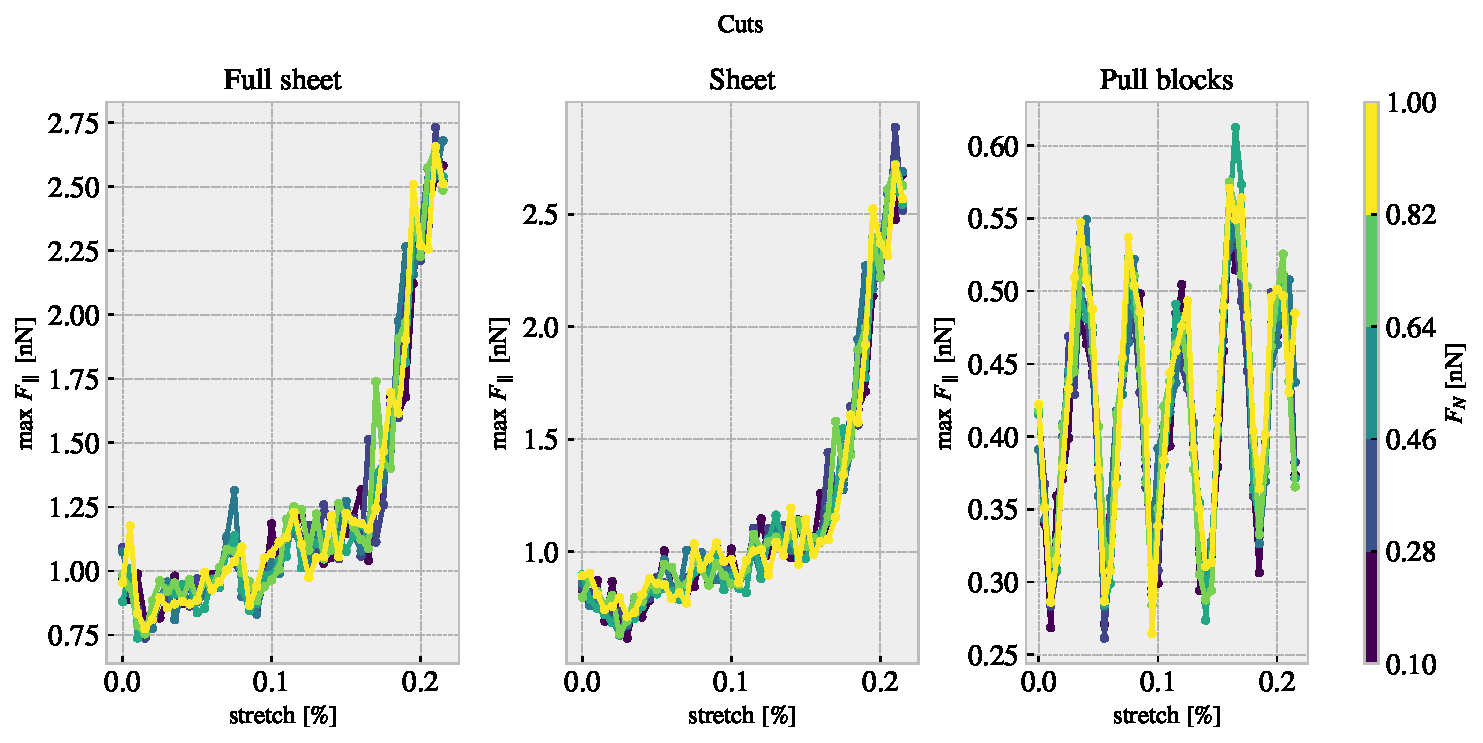
\includegraphics[width=\linewidth]{figures/max_group.pdf}
		\caption{Max friction for different parts of the cutted sheet, $F_N = [0.1, 1]$.}
	\end{figure}

\end{frame}



\begin{frame}
	\frametitle{Stage 2 - MD measurements}
	\framesubtitle{Frenkel-Kontorova Model}

	Friction force dependence of stretch might be explained by simple friction models such as the Frenkel-Kontorova (FK) model.

	\begin{align*}
		H=\sum_{i=1}^N\left[\frac{p_i^2}{2 m}+\frac{1}{2} K\left(x_{i+1}-x_i-a_c\right)^2+\frac{1}{2} U_0 \cos \frac{2 \pi x_i}{a_b}\right]
	\end{align*}
	\begin{figure}
		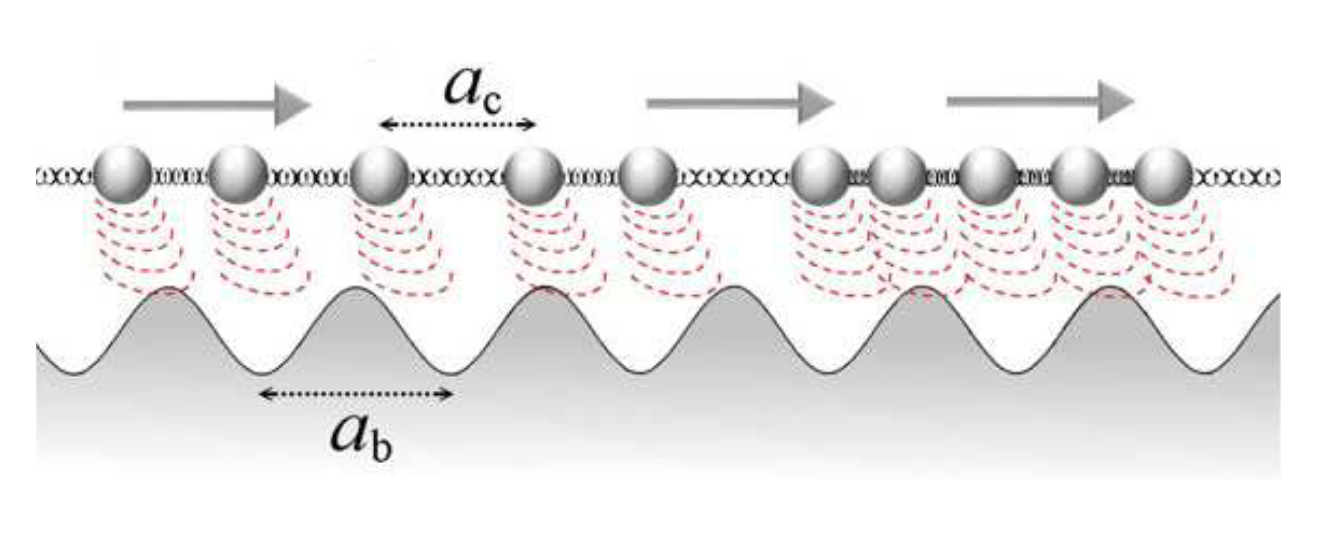
\includegraphics[width=0.65\linewidth]{figures/FK_model.png}
		\caption{A sketch of the FK model, showing the two competing lengths: The average interparticle spacing and the lattice periodicity of the substrate (Friction and Nonlinear Dynamics, N. Manini, 2016).}
	\end{figure}

\end{frame}




\begin{frame}[plain] % The optional argument 'plain' hides the headline and footline
	\begin{center}
		{\LARGE Questions? Comments?}
	\end{center}
\end{frame}


% \begin{frame}[plain] % The optional argument 'plain' hides the headline and footline
% 	\begin{center}
% 		{\Huge The End}
		
% 		\bigskip\bigskip % Vertical whitespace
		
% 		{\LARGE Questions? Comments?}
% 	\end{center}
% \end{frame}





%------------------------------------------------
%------------------------------------------------
%------------------------------------------------
%------------------------------------------------
%------------------------------------------------
%------------------------------------------------
%------------------------------------------------
%------------------------------------------------
%------------------------------------------------




% \begin{frame}
% 	\frametitle{Motivation}
	
% 	\begin{itemize}
% 		\item Friction has a huge impact in various engineering applications.
% 		\item Most obvious advantages: Energy efficiency
% 	\end{itemize}


% 	\begin{exampleblock}{}
% 		{``The economic aspects of tribology are significant. Investigations by a number of countries arrived at figures of savings of 1.0\% to 1.4\% of the GNPs, obtainable by the application of tribological principles.''}
% 		\vskip5mm
% 		\hspace*\fill{\tiny --- Professor H. Peter Jost, President, International Tribology Council}
% 	\end{exampleblock}

	
% \end{frame}






%------------------------------------------------



% \section{Methodology}

% % MD
% % Machine learning


% \section{Text Examples} % Sections are added in order to organize your presentation into discrete blocks, all sections and subsections are automatically output to the table of contents as an overview of the talk but NOT output in the presentation as separate slides

% %------------------------------------------------

% \subsection{Paragraphs and Lists}

% \begin{frame}
% 	\frametitle{Paragraphs of Text}
	
% 	Sed iaculis \alert{dapibus gravida}. Morbi sed tortor erat, nec interdum arcu. Sed id lorem lectus. Quisque viverra augue id sem ornare non aliquam nibh tristique. Aenean in ligula nisl. Nulla sed tellus ipsum. Donec vestibulum ligula non lorem vulputate fermentum accumsan neque mollis.
	
% 	\bigskip % Vertical whitespace
	
% 	% Quote example
% 	\begin{quote}
% 		Sed diam enim, sagittis nec condimentum sit amet, ullamcorper sit amet libero. Aliquam vel dui orci, a porta odio.\\
% 		--- Someone, somewhere\ldots
% 	\end{quote}
	
% 	\bigskip % Vertical whitespace
	
% 	Nullam id suscipit ipsum. Aenean lobortis commodo sem, ut commodo leo gravida vitae. Pellentesque vehicula ante iaculis arcu pretium rutrum eget sit amet purus. Integer ornare nulla quis neque ultrices lobortis.
% \end{frame}

% %------------------------------------------------

% \begin{frame}
% 	\frametitle{Lists}
% 	\framesubtitle{Bullet Points and Numbered Lists} % Optional subtitle
	
% 	\begin{itemize}
% 		\item Lorem ipsum dolor sit amet, consectetur adipiscing elit
% 		\item Aliquam blandit faucibus nisi, sit amet dapibus enim tempus
% 		\begin{itemize}
% 			\item Lorem ipsum dolor sit amet, consectetur adipiscing elit
% 			\item Nam cursus est eget velit posuere pellentesque
% 		\end{itemize}
% 		\item Nulla commodo, erat quis gravida posuere, elit lacus lobortis est, quis porttitor odio mauris at libero
% 	\end{itemize}
	
% 	\bigskip % Vertical whitespace
	
% 	\begin{enumerate}
% 		\item Nam cursus est eget velit posuere pellentesque
% 		\item Vestibulum faucibus velit a augue condimentum quis convallis nulla gravida 
% 	\end{enumerate}
% \end{frame}

% %------------------------------------------------

% \subsection{Blocks}

% \begin{frame}
% 	\frametitle{Blocks of Highlighted Text}
	
% 	\begin{block}{Block Title}
% 		Lorem ipsum dolor sit amet, consectetur adipiscing elit. Integer lectus nisl, ultricies in feugiat rutrum, porttitor sit amet augue.
% 	\end{block}
	
% 	\begin{exampleblock}{Example Block Title}
% 		Aliquam ut tortor mauris. Sed volutpat ante purus, quis accumsan.
% 	\end{exampleblock}
	
% 	\begin{alertblock}{Alert Block Title}
% 		Pellentesque sed tellus purus. Class aptent taciti sociosqu ad litora torquent per conubia nostra, per inceptos himenaeos.
% 	\end{alertblock}
	
% 	\begin{block}{} % Block without title
% 		Suspendisse tincidunt sagittis gravida. Curabitur condimentum, enim sed venenatis rutrum, ipsum neque consectetur orci.
% 	\end{block}
% \end{frame}

% %------------------------------------------------

% \subsection{Columns}

% \begin{frame}
% 	\frametitle{Multiple Columns}
% 	\framesubtitle{Subtitle} % Optional subtitle
	
% 	\begin{columns}[c] % The "c" option specifies centered vertical alignment while the "t" option is used for top vertical alignment
% 		\begin{column}{0.45\textwidth} % Left column width
% 			\textbf{Heading}
% 			\begin{enumerate}
% 				\item Statement
% 				\item Explanation
% 				\item Example
% 			\end{enumerate}
% 		\end{column}
% 		\begin{column}{0.5\textwidth} % Right column width
% 			Lorem ipsum dolor sit amet, consectetur adipiscing elit. Integer lectus nisl, ultricies in feugiat rutrum, porttitor sit amet augue. Aliquam ut tortor mauris. Sed volutpat ante purus, quis accumsan dolor.
% 		\end{column}
% 	\end{columns}
% \end{frame}

% %------------------------------------------------

% \section{Table and Figure Examples}

% \subsection{Table}

% \begin{frame}
% 	\frametitle{Table}
% 	\framesubtitle{Subtitle} % Optional subtitle
	
% 	\begin{table}
% 		\begin{tabular}{l l l}
% 			\toprule
% 			\textbf{Treatments} & \textbf{Response 1} & \textbf{Response 2}\\
% 			\midrule
% 			Treatment 1 & 0.0003262 & 0.562 \\
% 			Treatment 2 & 0.0015681 & 0.910 \\
% 			Treatment 3 & 0.0009271 & 0.296 \\
% 			\bottomrule
% 		\end{tabular}
% 		\caption{Table caption}
% 	\end{table}
% \end{frame}


% \section{Mathematics}

% \begin{frame}
% 	\frametitle{Definitions \& Examples}
	
% 	\begin{definition}
% 		A \alert{prime number} is a number that has exactly two divisors.
% 	\end{definition}
	
% 	\smallskip % Vertical whitespace
	
% 	\begin{example}
% 		\begin{itemize}
% 			\item 2 is prime (two divisors: 1 and 2).
% 			\item 3 is prime (two divisors: 1 and 3).
% 			\item 4 is not prime (\alert{three} divisors: 1, 2, and 4).
% 		\end{itemize}
% 	\end{example}
	
% 	\smallskip % Vertical whitespace
	
% 	You can also use the \texttt{theorem}, \texttt{lemma}, \texttt{proof} and \texttt{corollary} environments.
% \end{frame}

% %------------------------------------------------

% \begin{frame}
% 	\frametitle{Theorem, Corollary \& Proof}
	
% 	\begin{theorem}[Mass--energy equivalence]
% 		$E = mc^2$
% 	\end{theorem}
	
% 	\begin{corollary}
% 		$x + y = y + x$
% 	\end{corollary}
	
% 	\begin{proof}
% 		$\omega + \phi = \epsilon$
% 	\end{proof}
% \end{frame}

% %------------------------------------------------

% \begin{frame}
% 	\frametitle{Equation}

% 	\begin{equation}
% 		\cos^3 \theta =\frac{1}{4}\cos\theta+\frac{3}{4}\cos 3\theta
% 	\end{equation}
% \end{frame}

% %------------------------------------------------

% \begin{frame}[fragile] % Need to use the fragile option when verbatim is used in the slide
% 	\frametitle{Verbatim}
	
% 	\begin{example}[Theorem Slide Code]
% 		\begin{verbatim}
% 			\begin{frame}
% 				\frametitle{Theorem}
% 				\begin{theorem}[Mass--energy equivalence]
% 					$E = mc^2$
% 				\end{theorem}
% 		\end{frame}\end{verbatim} % Must be on the same line
% 	\end{example}
% \end{frame}

% %------------------------------------------------

% \begin{frame}
% 	Slide without title.
% \end{frame}

% %------------------------------------------------

% \section{Referencing}

% \begin{frame}
% 	\frametitle{Citing References}
	
% 	An example of the \texttt{\textbackslash cite} command to cite within the presentation:
	
% 	\bigskip % Vertical whitespace
	
% 	This statement requires citation \cite{p1,p2}.
% \end{frame}

% %------------------------------------------------

% \begin{frame} % Use [allowframebreaks] to allow automatic splitting across slides if the content is too long
% 	\frametitle{References}
	
% 	\begin{thebibliography}{99} % Beamer does not support BibTeX so references must be inserted manually as below, you may need to use multiple columns and/or reduce the font size further if you have many references
% 		\footnotesize % Reduce the font size in the bibliography
		
% 		\bibitem[Smith, 2022]{p1}
% 			John Smith (2022)
% 			\newblock Publication title
% 			\newblock \emph{Journal Name} 12(3), 45 -- 678.
			
% 		\bibitem[Kennedy, 2023]{p2}
% 			Annabelle Kennedy (2023)
% 			\newblock Publication title
% 			\newblock \emph{Journal Name} 12(3), 45 -- 678.
% 	\end{thebibliography}
% \end{frame}

% %----------------------------------------------------------------------------------------
% %	ACKNOWLEDGMENTS SLIDE
% %----------------------------------------------------------------------------------------

% \begin{frame}
% 	\frametitle{Acknowledgements}
	
% 	\begin{columns}[t] % The "c" option specifies centered vertical alignment while the "t" option is used for top vertical alignment
% 		\begin{column}{0.45\textwidth} % Left column width
% 			\textbf{Smith Lab}
% 			\begin{itemize}
% 				\item Alice Smith
% 				\item Devon Brown
% 			\end{itemize}
% 			\textbf{Cook Lab}
% 			\begin{itemize}
% 				\item Margaret
% 				\item Jennifer
% 				\item Yuan
% 			\end{itemize}
% 		\end{column}		
% 		\begin{column}{0.5\textwidth} % Right column width
% 			\textbf{Funding}
% 			\begin{itemize}
% 				\item British Royal Navy
% 				\item Norwegian Government
% 			\end{itemize}
% 		\end{column}
% 	\end{columns}
% \end{frame}

% %----------------------------------------------------------------------------------------
% %	CLOSING SLIDE
% %----------------------------------------------------------------------------------------

% \begin{frame}[plain] % The optional argument 'plain' hides the headline and footline
% 	\begin{center}
% 		{\Huge The End}
		
% 		\bigskip\bigskip % Vertical whitespace
		
% 		{\LARGE Questions? Comments?}
% 	\end{center}
% \end{frame}

%----------------------------------------------------------------------------------------

\end{document} 